\documentclass[11pt,a4paper]{article}
\usepackage[T1]{fontenc}
\usepackage{lmodern}
\usepackage[margin=27mm,headheight=15pt]{geometry}
\usepackage{amsmath,amssymb,amsthm,mathtools}
\usepackage{booktabs,array,longtable}
\usepackage{xcolor,tikz,microtype,enumitem,fancyhdr,hyperref}
\usetikzlibrary{arrows.meta,positioning}
\hypersetup{colorlinks=true,linkcolor=blue!45!black,citecolor=blue!45!black,
 urlcolor=blue!45!black,pdftitle={Explicit irrationality bounds for odd powers of pi},
 pdfauthor={Expository research notes}}
\setlength{\parskip}{4pt}
\setlength{\parindent}{1.2em}
\setlength{\emergencystretch}{2em}
\setlist{itemsep=3pt,topsep=5pt}
\allowdisplaybreaks[2]
\numberwithin{equation}{section}
\newtheorem{theorem}{Theorem}[section]
\newtheorem{lemma}[theorem]{Lemma}
\newtheorem{proposition}[theorem]{Proposition}
\newtheorem{corollary}[theorem]{Corollary}
\theoremstyle{definition}
\newtheorem{definition}[theorem]{Definition}
\newtheorem{example}[theorem]{Example}
\theoremstyle{remark}
\newtheorem{remark}[theorem]{Remark}
\newcommand{\ii}{\mathrm{i}}
\newcommand{\ZZ}{\mathbb Z}
\newcommand{\QQ}{\mathbb Q}
\newcommand{\NN}{\mathbb N}
\newcommand{\CC}{\mathbb C}
\newcommand{\dd}{\,\mathrm{d}}
\newcommand{\Hgt}{\mathrm H}
\newcommand{\LNNbound}{\frac{12970477737}{11706979}}
\DeclareMathOperator{\lcm}{lcm}
\DeclareMathOperator{\Res}{Res}
\DeclareMathOperator{\ord}{ord}
\pagestyle{fancy}
\fancyhf{}
\fancyhead[L]{\small Odd powers of \(\pi\)}
\fancyhead[R]{\small Expository research notes}
\fancyfoot[C]{\thepage}
\renewcommand{\headrulewidth}{0.3pt}
\begin{document}
\begin{titlepage}
\thispagestyle{empty}
\vspace*{15mm}
\begin{center}
{\LARGE\bfseries Explicit irrationality bounds\\[5pt]
for odd powers of \(\boldsymbol{\pi}\)}\\[9mm]
{\large Nested logarithmic Hermite--Pad\'e constructions,\\
prime divisors, and algebraic-approximation transfer}\\[12mm]
{\large Expository research notes}\\[3mm]
Revised 31 October 2026
\end{center}
\vspace{9mm}
\begin{abstract}
We develop a nested-interval version of a classical logarithmic
Hermite--Pad\'e construction and give explicit upper bounds for the
irrationality exponents of odd powers of \(\pi\). The construction uses
Gaussian-integer polynomials in \(\log\ii=\ii\pi/2\), rather than a
direct sequence of binary linear forms in \(1,\pi^k\).
We prove integrality, an exact nonvanishing determinant identity, a
prime-divisor estimate described by weighted arcs on a circle, and
uniform analytic bounds. A minimal-polynomial resultant argument
handles every rational approximation, including reducible-binomial
and rational-power cases. The latest twenty-eight-layer choice gives
\[
 \boxed{\mu(\pi^3)\le\LNNbound
 =1107.9269670681\ldots<1107.93.}
\]
This fixed result, including the actual auxiliary family and the required
arithmetic and analytic bounds, has an accepted Lean formalization.
The general transfer applies to every integer power \(k\ge2\); further
numerical instances and an explicit all-power recipe are explained with
their separate verification status. We also derive an older all-power
bound from Nesterenko--Waldschmidt and compare the even case with the
specialized bound for \(\zeta(4)\). Background, intermediate calculations,
worked examples, and a guide to the formal proof are included.
\end{abstract}
\vfill
\noindent\textbf{Status and scope.}
This is an expanded working manuscript, not a journal submission or an
independently refereed paper. It makes no priority, record, or global
optimality claim. The displayed upper bounds follow from the arguments
given here; finite tests and numerical certificates have more limited
roles, which are stated explicitly. No upper bound below \(100\) for
\(\mu(\pi^3)\) is established.
The exact L99 theorem is accepted locally; the entire expanded exposition
and every additional example are not thereby claimed to be formalized.
\end{titlepage}
\begingroup
\small
\setlength{\parskip}{0pt}
\tableofcontents
\endgroup
\clearpage
\section{Purpose, conventions, and main conclusions}

\subsection{What is being bounded?}

For an irrational real number \(\xi\), its irrationality exponent is
\[
\mu(\xi)=\sup\left\{u>0:
0<\left|\xi-\frac pq\right|<q^{-u}
\text{ for infinitely many reduced }p/q,\ q>0\right\}.
\]
Thus \(\mu(\xi)\le E\) means that for every \(\varepsilon>0\) there are
only finitely many reduced fractions with error below
\(q^{-E-\varepsilon}\). Equivalently, after changing a positive
constant, one has
\begin{equation}\label{eq:measuremeaning}
\left|\xi-\frac pq\right|\ge c_\varepsilon q^{-E-\varepsilon}
\end{equation}
for all \(p,q\) with \(q>0\). This does not assert the same inequality
with exponent exactly \(E\).

Dirichlet's theorem gives \(\mu(\xi)\ge2\). Obtaining an explicit upper
bound for a particular transcendental number is a separate problem.
The finiteness of the exponents of fixed powers of \(\pi\) is already
accessible through classical quantitative transcendence theory.
Our objective is to spell out one concrete construction and track
its constants, not to claim a first finiteness theorem.

All logarithms in estimates are natural logarithms. We use
\[
\lambda=\log\ii=\frac{\ii\pi}{2},\qquad \Theta=\frac\pi2.
\]
The symbols \(o(n)\) and \(O(\log n)\) refer to \(n\to\infty\)
with the complete interval configuration and target \(k\) fixed.
The auxiliary degree \(m\) may be large, but is fixed in this limit.

\subsection{Why odd powers are natural targets}

The Dirichlet beta function is
\[
\beta(s)=\sum_{\ell=0}^{\infty}\frac{(-1)^\ell}{(2\ell+1)^s}.
\]
For \(r\ge0\),
\[
\beta(2r+1)=
\frac{(-1)^r E_{2r}}{4^{r+1}(2r)!}\pi^{2r+1},
\]
where \(\operatorname{sech}z=\sum_{j\ge0}E_jz^j/j!\) defines the
Euler numbers. In particular,
\[
\beta(1)=\frac\pi4,\qquad
\beta(3)=\frac{\pi^3}{32},\qquad
\beta(5)=\frac{5\pi^5}{1536}.
\]
Multiplication by a nonzero rational number preserves the irrationality
exponent. For a reduced multiplier \(a/b\), reducing \(ap/(bq)\)
cancels a gcd dividing \(|ab|\), so its denominator remains comparable
to \(q\) by constants independent of \(p,q\).

This observation does \emph{not} deduce an upper bound for \(\pi^3\)
from a rational-approximation bound for \(\pi\). Taking a cube root
changes the approximation field. The resultant argument below accounts
for that change.

\subsection{A preview of the construction}

There are three components:
\begin{enumerate}
\item Build integer polynomials \(A_{h,j,n}(x)\) such that
\[
R_{h,n}(x)=\sum_{j=0}^{m}A_{h,j,n}(x)(\log x)^j
\]
has a high-order zero at \(x=1\).
\item Divide every coefficient by a common integer \(\Pi_n\).
Its exponential rate \(\gamma=\lim n^{-1}\log\Pi_n\) matters;
a large constant depending only on \(m\) does not change this rate.
\item Evaluate at \(x=\ii\), compare \(\lambda\) with a \(k\)-th root
of a rational approximation to \(\pi^k\), and use a nonzero resultant.
\end{enumerate}
Nested intervals change both analytic bounds and arithmetic divisors.
Their effects must be assessed together.

The classical logarithmic construction appears in
Mignotte~\cite{Mignotte}. Weighted logarithmic Pad\'e systems and
normality are discussed in Kawashima~\cite{Kawashima}.
Here the determinant and estimates for our two-sided nested system
are proved directly.

\subsection{General parameter theorem}

Choose integers
\[
L\ge3,\quad 0=t_0<t_1<\cdots<t_{J-1}<L/2,\quad \nu_j\ge1,
\]
and put
\[
M=\sum_{j=0}^{J-1}\nu_j,\qquad m=M-1\ge1,\qquad
c_j=1-\frac{2t_j}{L}.
\]
An interval of relative length \(c_j\), centred at \(1/2\), is used
\(\nu_j\) times. Let \(\gamma\) be the explicit prime-divisor rate
defined in Section~\ref{sec:arithmetic}. Let \(Y>0\) solve
\begin{equation}\label{eq:rootpreview}
2\sum_j\nu_j\arctan\frac{c_j}{2Y}=\Theta.
\end{equation}
Define
\begin{align}
F_c(Y)&=\frac c2\log\frac{1+(2Y/c)^2}{4}
             +2Y\arctan\frac{c}{2Y},\label{eq:Fdef}\\
D_0&=\sum_j\nu_jF_{c_j}(Y)-\Theta Y-m,\label{eq:D0def}\\
G_0&=m+\left(\sum_j\nu_jc_j\right)\log2,\label{eq:G0def}\\
D&=D_0+\gamma,\qquad G=G_0-\gamma.\label{eq:DGdef}
\end{align}

\begin{theorem}[Odd-power bound]\label{thm:main}
Let \(k\ge3\) be odd. If \(G\ge0\) and
\(\Delta_k=D-(k-1)G>0\), then
\begin{equation}\label{eq:mainbound}
\boxed{\displaystyle
\mu(\pi^k)\le E_k:=
\frac{m(D+G)}{D-(k-1)G}
=\frac{m(D_0+G_0)}
 {D_0-(k-1)G_0+k\gamma}.}
\end{equation}
\end{theorem}

The proof also works for every integer \(k\ge2\). We emphasize odd
powers because they are the motivating targets; we do not compare
these bounds with specialized results for even powers.

\begin{corollary}[A twelve-layer family]\label{cor:numerical}
Use \(L=69\), \(t_j=j\) for \(0\le j\le11\), and
\[
\nu_0=6s,\qquad \nu_1=\cdots=\nu_{11}=s,\qquad m=17s-1.
\]
The following choices satisfy the hypotheses:
\begin{center}
\begin{tabular}{rrrr}
\toprule
\(k\)&\(s\)&\(m\)&Certified strict upper bound\\
\midrule
3&11&186&\(1203.973\)\\
5&259&\(4\,402\)&\(42\,461\)\\
7&\(5\,871\)&\(99\,806\)&\(1\,272\,103\)\\
9&\(131\,354\)&\(2\,233\,017\)&\(35\,398\,937\)\\
\bottomrule
\end{tabular}
\end{center}
For every other fixed odd \(k\), some sufficiently large integer \(s\)
also satisfies the hypotheses.
\end{corollary}

The last assertion is an existence statement within an explicit
family, not a uniform small bound as \(k\to\infty\).
Section~\ref{sec:parameters} explains the growth.

\subsection{A guide to the evidence}

The algebraic and analytic lemmas prove Theorem~\ref{thm:main}.
Ball-arithmetic certificates prove the decimal comparisons once the
lemmas hold. Exact finite examples check identities and implementation,
but do not prove asymptotic rates. Floating-point searches select
parameters; they neither certify rounding nor prove global optimality.
The appendices retain unsuccessful experiments because they explain
the arithmetic difficulties that remain.

\section{Background and a reading guide}
\label{sec:background}

\subsection{Irrationality, transcendence, and approximation are different questions}

An irrationality proof rules out an equality \(\xi=p/q\).
An irrationality-exponent bound rules out an unlimited supply of
exceptionally accurate near-equalities. Transcendence rules out all
polynomial equalities with integer coefficients, but by itself does
not quantify how small a nonzero polynomial value may be. The last
distinction is essential here: the transcendence of \(\pi\) already
implies that \(\pi^k\) is irrational for every positive integer \(k\),
yet it does not supply the numerical exponent in
\eqref{eq:measuremeaning}.

For example, the statement \(\mu(\xi)\le E\) controls infinitely many
denominator scales. A long continued-fraction computation supplies
finitely many very good approximations, and may reveal useful
patterns, but cannot exclude a new pattern at larger denominators.
The present proof therefore constructs auxiliary objects for every
sufficiently large index \(n\), and relates that index to an arbitrary
denominator \(q\). This is the reason for the uniformity requirements
in Sections~\ref{sec:analysis} and~\ref{sec:transfer}.

It is also useful to separate three quantities often called a
``measure.'' A numerical exponent \(E\) specifies the power of \(q\).
A positive prefactor \(c_\varepsilon\) specifies the scale of the lower
bound. A denominator threshold \(q_0(\varepsilon)\) specifies where
that lower bound starts. These notes make \(E\) explicit, but do not
tabulate numerical values for the other two quantities in the nested
construction. Allowing an arbitrary positive exponent slack is part
of the theorem, not a rounding convention.

\subsection{What Pad\'e approximation contributes}

For a power series \(f(x)\), ordinary Pad\'e approximation seeks
polynomials \(P,Q\) for which \(Q(x)f(x)-P(x)\) has a prescribed
high-order zero. Hermite--Pad\'e approximation replaces a single
function by several functions. In our setting these are
\[
1,\log x,(\log x)^2,\ldots,(\log x)^m.
\]
For each row \(h\), the expression
\[
R_{h,n}(x)=A_{h,0,n}(x)+A_{h,1,n}(x)\log x
 +\cdots+A_{h,m,n}(x)(\log x)^m
\]
vanishes to high order at \(x=1\). At a fixed evaluation point this
can make its value small even though its coefficients are large.
The integral representation is an efficient way to impose many
vanishing conditions simultaneously.

The vanishing conditions are linear equations, but solving a large
rational linear system independently at every \(n\) would conceal
the denominators and make nonvanishing difficult to track. The
explicit rational kernel instead exposes its poles, factorials,
and local expansions. These are exactly the objects needed later
for integrality and prime-divisor estimates.

There are \(m+1\) rows because a single small polynomial may vanish
at the algebraic number selected by a rational approximation.
An invertible coefficient matrix ensures that the entire family
cannot vanish there. The exact determinant is therefore an
arithmetic selection tool: it supplies at least one useful row at
every denominator scale.

\subsection{Why evaluate at a complex point?}

The principal logarithm at \(\ii\) is
\(\lambda=\ii\pi/2\), so powers of the logarithm encode powers of
\(\pi\). An integer polynomial evaluated at \(\ii\) has coefficients
in \(\ZZ[\ii]\), a ring whose nonzero elements have modulus at
least one. This discreteness replaces the familiar lower bound
\(|a|\ge1\) for a nonzero ordinary integer.

No irrationality conclusion follows merely from making
\(U_{h,n}(\lambda)\) small: its degree is usually much larger than
the target power \(k\). The next step is to compare it with
\(U_{h,n}(y)\), where
\[
y=\frac{\ii}{2}(p/q)^{1/k}
\]
is algebraic. The comparison is useful because an algebraic value
has a nonzero integral resultant, while the logarithmic value is
small by analysis. The divided difference controls the cost of
moving from \(\lambda\) to \(y\).

For odd powers, an alternative motivation comes from the rational
multiple \(\beta(2r+1)/\pi^{2r+1}\). That identity suggests trying
binary linear forms in \(1,\beta(3)\), but it does not require us
to find them. The present method uses a higher-dimensional system
and a resultant instead. The unsuccessful binary experiments in
Appendix~\ref{app:experiments} explain why this detour was useful.

\subsection{The two parameters that must not be interchanged}

The interval configuration, its multiplicities, and \(m\) are fixed
before the limit \(n\to\infty\). The index \(n\), taken through
multiples of \(L\), determines the number of poles in the rational
kernel. The degree \(m\) determines the number of logarithmic powers
and rows. They have different roles even when both are large.

For instance, in the accepted L99 application \(m=171\), whereas
\(n\) is unbounded. A factor \(171!\) is a constant with respect
to \(n\), so its logarithm divided by \(n\) tends to zero. A
factor \(d_n^{171}\) is not a constant: its exponential rate is
\(171\). Treating these two factors alike can easily reverse the
apparent success of a construction.

When the target power \(k\) changes, we may select another fixed
scale \(s\), hence another fixed \(m\). The all-power theorem means
that this can be done for each \(k\), followed by the separate
limit in \(n\). It does not authorize a simultaneous limit
\(k=k(n)\) in the estimates already proved.

\subsection{A map of the proof}

\begin{figure}[ht]
\centering
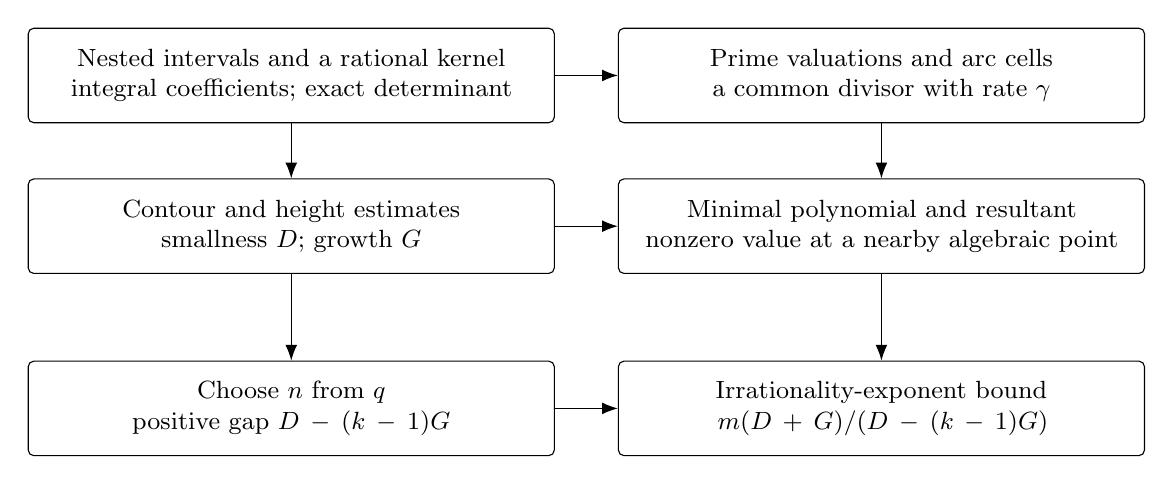
\begin{tikzpicture}[
 box/.style={draw,rounded corners=2pt,align=center,text width=64mm,
 minimum height=12mm,inner sep=4pt,font=\small},
 >={Latex[length=2mm]},node distance=7mm and 8mm]
\node[box] (a) {Nested intervals and a rational kernel\\
integral coefficients; exact determinant};
\node[box,right=of a] (b) {Prime valuations and arc cells\\
a common divisor with rate \(\gamma\)};
\node[box,below=of a] (c) {Contour and height estimates\\
smallness \(D\); growth \(G\)};
\node[box,below=of b] (d) {Minimal polynomial and resultant\\
nonzero value at a nearby algebraic point};
\node[box,below=11mm of c,text width=64mm] (e)
 {Choose \(n\) from \(q\)\\
positive gap \(D-(k-1)G\)};
\node[box,right=of e] (f) {Irrationality-exponent bound\\
\(m(D+G)/(D-(k-1)G)\)};
\draw[->] (a)--(b);
\draw[->] (a)--(c);
\draw[->] (b)--(d);
\draw[->] (c)--(d);
\draw[->] (c)--(e);
\draw[->] (d)--(f);
\draw[->] (e)--(f);
\end{tikzpicture}
\caption{The proof separates construction, arithmetic, analysis, and
transfer. A numerical improvement must respect all four parts.}
\label{fig:proofmap}
\end{figure}

A first reading can follow the overview, the L99 ledger in
Section~\ref{subsec:l99}, and the transfer proof. A second reading
can fill in the local coefficient expansion and the contour tails.
The arc partition and the formalization guide are best read after
the purpose of a common divisor is clear. Appendix~\ref{app:reader}
collects notation and short checks that can be carried out by hand.

The main prerequisites are elementary complex analysis, polynomial
algebra over \(\QQ\) and \(\QQ(\ii)\), prime valuations, and
asymptotic estimates. Resultants, confluent Vandermonde matrices,
and interval arithmetic are introduced where they enter the proof.
Knowledge of Lean is not required to read the mathematical argument.

\section{Prior explicit bounds and the even-power comparison}
\label{sec:literature}

\subsection{An older theorem already gives a number for every power}

The distinction between an explicitly tabulated bound and a bound
that follows by substitution into a general theorem matters here.
Nesterenko--Waldschmidt~\cite{NesterenkoWaldschmidt}, Theorem~2(1),
prove that if \(\xi\) is real algebraic of degree \(d\) and
coefficient length at most \(\mathcal L\ge3\), then
\begin{equation}\label{eq:NW}
|\pi-\xi|\ge
\exp\{-1200000d(\log\mathcal L+d\log d)(1+\log d)\}.
\end{equation}
The coefficient length of an integral polynomial is the sum of the
absolute values of its coefficients; for an algebraic number it is
the length of its primitive integral minimal polynomial. The
following specialization is derived here from their theorem.

\begin{proposition}[A classical all-power consequence]\label{prop:NWpowers}
For every integer \(k\ge1\), put
\[
B(k)=1200000k(1+\log k).
\]
Then \(\mu(\pi^k)\le B(k)\). In particular, explicit exponent
upper bounds for all fixed powers were already available from
classical quantitative transcendence theory.
\end{proposition}
\begin{proof}
It suffices first to consider \(q\ge1\) and
\(|\pi^k-p/q|<1\). This implies \(p/q>0\). Set
\(\theta=(p/q)^{1/k}\), and let \(f\) be its primitive integral
minimal polynomial, of degree \(d\le k\) and positive leading
coefficient \(a\). Gauss's lemma gives
\(f\mid qX^k-p\) in \(\ZZ[X]\), after removing the content of
the latter polynomial if necessary. In particular \(a\le q\).
Every conjugate of \(\theta\) is a root of this binomial, hence
has modulus \(\theta\). Also \(\theta<\pi+1\). The elementary
bound for the coefficients of a product gives
\[
\mathcal L(f)\le a(1+\theta)^d<6^kq.
\]
This step uses the minimal polynomial and remains valid when the
binomial is reducible.

Use \(\mathcal L=6^kq\) in \eqref{eq:NW}. Monotonicity in
\(1\le d\le k\) yields
\[
|\pi-\theta|\ge
\exp\{-B(k)(\log q+k\log6+k\log k)\}
=(6k)^{-kB(k)}q^{-B(k)}.
\]
Finally,
\[
|\pi^k-p/q|=|\pi-\theta|
 \sum_{a=0}^{k-1}\pi^{k-1-a}\theta^a
\ge\pi^{k-1}|\pi-\theta|.
\]
For the fractions excluded at the start the error is at least one.
Thus the smaller prefactor \((6k)^{-kB(k)}\) gives a lower bound
for all integer \(p\) and \(q\ge1\), proving the exponent claim.
\end{proof}

This consequence is not a claim that the original paper prints a
table of \(\pi^k\) exponents. It shows why absence of such a table
would not establish priority for an explicit number. It also gives
an independent comparison whose growth is only \(O(k\log k)\).

\begin{center}
\begin{tabular}{rrr}
\toprule
\(k\)&Classical consequence \(B(k)\), approximately
 &Bound displayed in these notes\\
\midrule
3&\(7\,555\,004.24\)&\(1107.93\)\\
5&\(15\,656\,627.47\)&\(42\,461\)\\
7&\(24\,745\,645.25\)&\(1\,272\,103\)\\
9&\(34\,530\,025.44\)&\(35\,398\,937\)\\
\bottomrule
\end{tabular}
\end{center}

The first three entries show a substantial improvement over this
particular classical consequence. The fourth does not: the old
general theorem already beats the displayed twelve-layer \(k=9\)
number. None of these comparisons is an exhaustive literature
search for the best bound at the indicated power. They delimit the
contribution that can safely be claimed.

\subsection{Even zeta values give an identification, not an approximation theorem}

Euler's formula, with \(B_{2r}\) the Bernoulli numbers, reads
\[
\zeta(2r)=\frac{(-1)^{r+1}B_{2r}(2\pi)^{2r}}{2(2r)!}
\in\QQ^\times\pi^{2r}.
\]
Therefore \(\mu(\zeta(2r))=\mu(\pi^{2r})\). For example,
\[
\zeta(2)=\pi^2/6,\qquad \zeta(4)=\pi^4/90.
\]
This equality transfers an existing irrationality-exponent estimate
between two names for the same rationally scaled constant. It does
not turn evaluation of the zeta value into a proof of a sharp
irrationality measure. Nor does an upper bound for \(\mu(\pi^2)\)
automatically give the corresponding upper bound for \(\mu(\pi^4)\).
Approximating \((\pi^2)^2\) and approximating \(\pi^2\) by rational
numbers are different approximation problems.

Marcovecchio--Zudilin~\cite{MarcovecchioZudilin} establish the
unconditional specialized estimate
\begin{equation}\label{eq:zeta4benchmark}
\mu(\pi^4)=\mu(\zeta(4))\le12.51085940\ldots.
\end{equation}
Their 2019 preprint, published in 2020, uses a different
hypergeometric representation to control the arithmetic of
approximations to \(\zeta(4)\). The bound does not assume the older
denominator conjecture discussed in their introduction. It is the
specialized benchmark verified for this revision; the present notes
do not claim a complete current classification of all later work.

\subsection{What the same L99 shape would do for the fourth power}

For the accepted cubic rates, direct substitution gives
\[
D-3G=544.69491-3(213.81256)=-96.74277.
\]
Thus the fixed accepted cubic instance is inadmissible for \(k=4\).
This is a failed hypothesis, rather than a failure of the general
transfer theorem. Increasing the common multiplicity scale changes
both the degree and the decay-to-height ratio.

For orientation, keep the base L99 shape
\((16,1,\ldots,1)\), and use the root-free lower rate of
Section~\ref{subsec:l99uniform} with scale \(s=19\). Then
\[
\begin{split}
m&=816,\qquad \underline D_s\approx3630.47940,\\
G_s&\approx1019.35966,\qquad
\underline D_s-3G_s\approx572.40043.
\end{split}
\]
The associated expression is approximately \(6628.69640\).
The accompanying numerical check certifies that it is below
\(6628.70\), using the already proved rational divisor lower rate.
This is a manuscript-level specialization and an Arb comparison,
not an accepted fixed Lean theorem for \(\pi^4\). Its size is
already sufficient to explain the comparison: the uniform method
is far from \eqref{eq:zeta4benchmark}.

Consequently there are two different useful projects. Completing
general-power applications tests and documents a reusable proof
framework. Improving the specialized fourth-power bound requires
competing below \(12.51085940\ldots\), most naturally by sharpening
the arithmetic of direct \(\zeta(4)\) approximations. Extending the
range of a theorem and improving the best numerical constant are
distinct achievements.

\section{The auxiliary polynomials and their determinant}
\label{sec:algebra}

\subsection{Intervals, poles, and normalization}

Fix the parameters of Theorem~\ref{thm:main}. Let \(n\) run through
positive multiples of \(L\). List all \(M=m+1\) intervals, including
repetitions, in nested order:
\[
I_a=[\alpha_a,\beta_a],\quad 0\le a\le m,\qquad
0=\alpha_0\le\cdots\le\alpha_m<n/2,\quad
\beta_a=n-\alpha_a.
\]
Thus \(I_m\subseteq\cdots\subseteq I_0=[0,n]\).
Write \(\ell_a=\beta_a-\alpha_a\).
The grouped description uses endpoints
\(t_jn/L,(L-t_j)n/L\), with multiplicity \(\nu_j\).

Set
\begin{equation}\label{eq:QandC}
\begin{split}
Q_n(z)&=\prod_{a=0}^{m}\prod_{r=\alpha_a}^{\beta_a}(z+r),\\
N_n&=\sum_{a=0}^{m}\ell_a,\qquad
d_n=\lcm(1,\ldots,n),\\
C_n&=m!\,d_n^m\prod_{a=0}^{m}\ell_a!.
\end{split}
\end{equation}
The degree of \(Q_n\) is \(N_n+M\).
\emph{The interval factorials are in the numerator of \(C_n\).}

Let \(\Gamma\) positively surround the poles \(0,-1,\ldots,-n\).
On a local logarithm branch define
\begin{equation}\label{eq:Rdef}
R_{h,n}(x)=\frac{C_n}{2\pi\ii}
\oint_\Gamma \frac{z^h x^{z+n}}{Q_n(z)}\dd z,\qquad 0\le h\le m.
\end{equation}
Write
\[
\frac{z^h}{Q_n(z)}
=\sum_{\ell=0}^{n}\sum_{r=1}^{\mu_\ell}
\frac{b_{h,\ell,r}}{(z+\ell)^r},
\quad
\mu_\ell=\#\{a:\ell\in I_a\}.
\]
Residues give
\begin{align}
R_{h,n}(x)&=\sum_{j=0}^{m}A_{h,j,n}(x)(\log x)^j,\label{eq:Rexpand}\\
A_{h,j,n}(x)&=\frac{C_n}{j!}
\sum_{\ell:\mu_\ell\ge j+1}
b_{h,\ell,j+1}x^{n-\ell}.\label{eq:Adef}
\end{align}

\subsection{Why all coefficients are integers}

\begin{lemma}[Integrality]\label{lem:integrality}
For all \(h,j\), one has \(A_{h,j,n}(x)\in\ZZ[x]\).
\end{lemma}
\begin{proof}
Absorb the interval factorials first:
\[
H_a(z)=\frac{\ell_a!}{\prod_{r=\alpha_a}^{\beta_a}(z+r)}.
\]
If \(\ell\in I_a\), expansion at \(z=-\ell+w\) gives
\begin{equation}\label{eq:polelocal}
wH_a(-\ell+w)=
(-1)^{\ell-\alpha_a}\binom{\ell_a}{\ell-\alpha_a}
\prod_{\substack{r\in I_a\\r\ne\ell}}
\left(1+\frac{w}{r-\ell}\right)^{-1}.
\end{equation}
The coefficient of \(w^u\) has denominator dividing \(d_n^u\):
every distance is a nonzero integer of absolute value at most \(n\).

If \(\ell\notin I_a\), use
\begin{equation}\label{eq:regularpartial}
H_a(z)=\sum_{r=\alpha_a}^{\beta_a}
\frac{(-1)^{r-\alpha_a}\binom{\ell_a}{r-\alpha_a}}{z+r}.
\end{equation}
Now the coefficient of \(w^u\) has denominator dividing \(d_n^{u+1}\).
The extra factor matters: a regular factor need not have an integral
constant term.

There are \(\mu_\ell\) pole factors and \(M-\mu_\ell\) regular factors.
The coefficient of \((z+\ell)^{-j-1}\) requires total local order
\(\mu_\ell-1-j\). The polynomial \((-\ell+w)^h\) has integer
coefficients and can only reduce the order required from the other
factors. Thus the necessary exponent of \(d_n\) is at most
\[
(\mu_\ell-1-j)+(M-\mu_\ell)=m-j.
\]
Multiplication by \(m!d_n^m/j!\) clears the denominators.
\end{proof}

The cancellation of \(\mu_\ell\) is why a variable pole multiplicity
does not require a larger universal power than \(d_n^m\).

\subsection{Supports and vanishing orders}

Nestedness implies
\[
\mu_\ell\ge j+1\quad\Longleftrightarrow\quad
\ell\in[\alpha_j,\beta_j].
\]
Hence \(A_{h,j,n}\) is divisible by \(x^{n-\beta_j}\), and the
remaining degree is at most \(\ell_j\).

\begin{lemma}[Vanishing at \(1\)]\label{lem:vanishing}
Every \(R_{h,n}\) has a zero of order at least \(N_n\) at \(x=1\).
\end{lemma}
\begin{proof}
Put \(w=\log x\). The coefficient of \(w^r\) in the integral of
\(z^h e^{zw}/Q_n(z)\) is zero whenever \(h+r\le\deg Q_n-2\), by the
residue at infinity. The first possible order is therefore
\[
\deg Q_n-h-1=N_n+M-h-1\ge N_n.
\]
Multiplication by \(x^n\) does not change this order.
Also \(\log x=(x-1)+O((x-1)^2)\).
\end{proof}

\subsection{A nonzero determinant, including its leading term}

\begin{proposition}[Exact determinant]\label{prop:det}
There exists \(c_n\ne0\) such that
\begin{equation}\label{eq:detidentity}
\det(A_{h,j,n}(x))_{0\le h,j\le m}
=c_n x^{\sum_j(n-\beta_j)}(x-1)^{N_n}.
\end{equation}
In particular \(A_n(\ii)\) is invertible.
\end{proposition}
\begin{proof}
The supports give the power of \(x\). After it is removed, the
determinant has degree at most \(N_n\).
Replace column zero by the sum of column \(j\) multiplied by
\((\log x)^j\), for \(0\le j\le m\).
Its determinant is unchanged; the new column consists of the
\(R_{h,n}(x)\). Lemma~\ref{lem:vanishing} supplies the factor
\((x-1)^{N_n}\).

To prove nonvanishing, take a block of repeated left endpoints
\[
\alpha_u=\cdots=\alpha_v=\alpha,\qquad r=v-u+1.
\]
The pole at \(-\alpha\) has multiplicity \(v+1\). Write
\[
\frac1{Q_n(-\alpha+w)}
=w^{-(v+1)}B_\alpha(w),\qquad B_\alpha(0)\ne0.
\]
For \(u\le j\le v\), the coefficient of \(x^{n-\alpha}\) in column
\(j\) is
\[
\frac{C_n}{j!}[w^{v-j}]
\bigl((-\alpha+w)^hB_\alpha(w)\bigr).
\]
The orders \(v-j\) are \(0,\ldots,r-1\), in reverse order.
Multiplication by \(B_\alpha\) gives an invertible triangular
change on these functionals.

In all blocks together, the leading-coefficient matrix reduces to
the divided-derivative evaluations of \(1,z,\ldots,z^m\) at distinct
points \(-\alpha\). This confluent Vandermonde matrix is invertible:
a polynomial in its kernel would have zeros of total multiplicity
\(M=m+1\), exceeding its degree. Thus the leading determinant is
nonzero, proving the identity.
\end{proof}

High vanishing order and a degree bound alone would also allow the
zero determinant. The leading-term argument rules out that possibility.

\section{Prime divisors and weighted zero arcs}
\label{sec:arithmetic}

\subsection{A local valuation inequality}

For a rational number \(u\ne0\), let \(\ord_p(u)\) be its usual
\(p\)-adic valuation, and put \(\ord_p(0)=+\infty\).
We only use primes \(\sqrt n<p\le n\), so a nonzero distance of
absolute value at most \(n\) has valuation at most one.

\begin{lemma}[A coefficientwise divisor]\label{lem:valuation}
For such a prime and an integer \(0\le\ell\le n\), put
\[
w_a(p,\ell)=
\left\lfloor\frac{\ell_a}{p}\right\rfloor
-\left\lfloor\frac{\ell-\alpha_a}{p}\right\rfloor
-\left\lfloor\frac{\beta_a-\ell}{p}\right\rfloor.
\]
Each \(w_a\) is \(0\) or \(1\). Every coefficient of \(x^{n-\ell}\)
in \(A_{h,j,n}\) has valuation at least
\begin{equation}\label{eq:valbound}
\sum_{a=0}^{m}w_a(p,\ell)+j.
\end{equation}
\end{lemma}
\begin{proof}
The assertion \(w_a\in\{0,1\}\) follows from
\(\lfloor u+v\rfloor-\lfloor u\rfloor-\lfloor v\rfloor\in\{0,1\}\),
with \(u=(\ell-\alpha_a)/p\) and \(v=(\beta_a-\ell)/p\).

For a pole factor, the constant in~\eqref{eq:polelocal} is a binomial
coefficient of valuation exactly \(w_a\), by the factorial valuation
formula and \(p^2>n\). Its coefficient of order \(u\) has valuation
at least \(w_a-u\).

For a regular factor the constant term has valuation \(w_a-1\).
For example, if \(\ell<\alpha_a\) and \(s=\alpha_a-\ell\), it equals
\[
H_a(-\ell)=\frac{\ell_a!(s-1)!}{(s+\ell_a)!}.
\]
Use
\(\lfloor(s-1)/p\rfloor=-\lfloor-s/p\rfloor-1\);
the other side of the interval is identical up to sign.
Expansion of the reciprocal linear factors loses at most one
valuation per order, so order \(u\) has valuation at least
\(w_a-1-u\).

The needed total order is at most \(\mu_\ell-1-j\), and there are
\(M-\mu_\ell\) regular factors. Since
\(\ord_p(d_n)=1\), the lower bound after multiplication by \(d_n^m\)
is
\[
m+\sum_aw_a-(M-\mu_\ell)-(\mu_\ell-1-j)
=\sum_aw_a+j.
\]
The factor \(m!/j!\) and coefficients of \((-\ell+w)^h\) are integers
and cannot lower this bound. Sums of terms preserve the lower bound.
\end{proof}

This estimate is stronger than needed. We discard the extra \(j\)
and minimize over the pole location in order to obtain a divisor
common to all entries of the matrix.

\subsection{Replacing pole locations by a circle}

Write \(n=LN_0\). For the grouped intervals define
\begin{equation}\label{eq:W}
W_j(z,y)=\lfloor(L-2t_j)z\rfloor
-\lfloor y-t_jz\rfloor-\lfloor(L-t_j)z-y\rfloor.
\end{equation}
It is periodic in \(z\) and \(y\) with period one and takes values
in \(\{0,1\}\). At \(z=N_0/p,\ y=\ell/p\), it is precisely the
local \(w_a\) for an interval of type \(j\).

For generic \(z\), the set on which \(W_j(z,y)=0\) is the closed
counterclockwise arc from \(\{t_jz\}\) to \(\{(L-t_j)z\}\).
Its length is \(\{(L-2t_j)z\}\), where braces denote fractional part.
Thus
\begin{equation}\label{eq:f}
f(z)=\min_{0\le y<1}\sum_j\nu_jW_j(z,y)
=M-\max_y\{\text{total weight of zero arcs containing }y\}.
\end{equation}
The weights are the interval multiplicities \(\nu_j\).

\begin{figure}[ht]
\centering
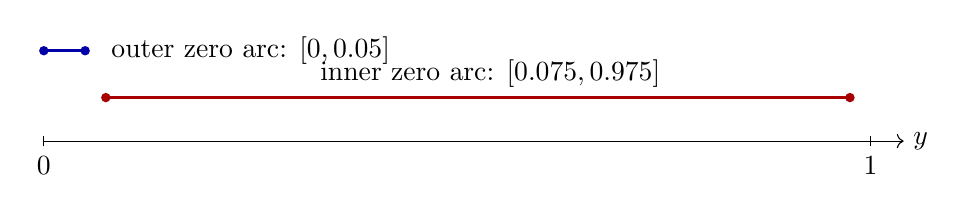
\begin{tikzpicture}[x=10.5cm,y=0.85cm]
\draw[->] (0,0)--(1.04,0) node[right]{\(y\)};
\foreach \x/\lab in {0/0,1/1}
{\draw (\x,-0.08)--(\x,0.08); \node[below] at (\x,-0.08){\(\lab\)};}
\draw[very thick,blue!65!black] (0,1.35)--(0.05,1.35);
\fill[blue!65!black] (0,1.35) circle (1.7pt);
\fill[blue!65!black] (0.05,1.35) circle (1.7pt);
\node[right] at (0.07,1.35){outer zero arc: \([0,0.05]\)};
\draw[very thick,red!65!black] (0.075,0.65)--(0.975,0.65);
\fill[red!65!black] (0.075,0.65) circle (1.7pt);
\fill[red!65!black] (0.975,0.65) circle (1.7pt);
\node[above] at (0.54,0.65){inner zero arc: \([0.075,0.975]\)};
\end{tikzpicture}
\caption{For \(L=14,\ t_0=0,\ t_1=1,\ z=3/40\), the zero arcs
are disjoint. With equal weights \(r\), their common-complement cost
is \(f(z)=r\): at least one type contributes \(r\) at every \(y\).}
\label{fig:arcs}
\end{figure}

All endpoints are affine integer multiples of \(z\), modulo one.
Their cyclic order changes only at the following finite rational set.
Let
\[
\mathcal S=\{0\}\cup\{t_j,L-t_j:0\le j<J\},\qquad
\mathcal D=\{|u-v|:u,v\in\mathcal S,\ u\ne v\}.
\]
Take all fractions \(a/d\in[0,1]\) with \(d\in\mathcal D\), remove
duplicates, and list them as
\[
0=u_0<u_1<\cdots<u_R=1.
\]
On each open interval \((u_r,u_{r+1})\), the integer \(f(z)\) is
constant. At a fixed rational midpoint \(z\), it can be calculated
exactly by checking midpoints between consecutive arc endpoints.
Off this exceptional set no distinct endpoints coincide, so an
endpoint cannot have a smaller value than both adjacent open arcs.

To avoid endpoint conventions entirely, define \(f=0\) at every
breakpoint and extend it periodically. This only weakens the local
divisor estimate and does not change any integral below.

\subsection{The common divisor and its exact exponential rate}

Define
\begin{equation}\label{eq:Pi}
\Pi_n=\prod_{\sqrt n<p\le n}p^{f(N_0/p)}.
\end{equation}
By Lemma~\ref{lem:valuation}, \(\Pi_n\) divides every integer
coefficient of every \(A_{h,j,n}(x)\). It is a rational integer;
we do not need factorization into Gaussian primes.

\begin{proposition}[Digamma formula]\label{prop:gamma}
The limit \(\gamma=\lim n^{-1}\log\Pi_n\) exists and is
\begin{equation}\label{eq:gamma}
\boxed{\displaystyle
\gamma=\frac1L\sum_{\substack{0\le r<R\\u_r>0}}
 f\!\left(\frac{u_r+u_{r+1}}2\right)
 \bigl(\psi(u_{r+1})-\psi(u_r)\bigr),}
\end{equation}
where \(\psi=\Gamma'/\Gamma\).
\end{proposition}
\begin{proof}
For all sufficiently small \(z>0\), none of the endpoints wraps
around the circle and the zero arcs are nested about \(Lz/2\).
They have a common point, so \(f(z)=0\). Thus the apparent singularity
at \(u_0=0\) contributes nothing.

For an interval \((a,b)\subset(0,1)\) on which \(f=v\), periodicity
selects primes satisfying
\[
N_0/(r+b)<p<N_0/(r+a),\qquad r=0,1,\ldots.
\]
For each fixed \(r\), the prime number theorem
\(\vartheta(X)=\sum_{p\le X}\log p=X+o(X)\) makes their contribution
to \(n^{-1}\log\Pi_n\) tend to
\[
\frac vL\left(\frac1{r+a}-\frac1{r+b}\right).
\]
The sum over \(r\ge T\) is bounded, uniformly in large \(n\), by a
constant times \(M/(LT)\), using the elementary Chebyshev bound
\(\vartheta(X)=O(X)\). Primes below \(\sqrt n\) contribute \(o(n)\).
These observations justify passage from finitely many periods to all
periods.

Breakpoint exclusions also cost only \(O(\log n)\). Indeed,
\(\{N_0/p\}=a/d\) implies that \(p\) divides \(dN_0\);
the denominators \(d\) belong to a fixed finite set.
Finally,
\[
\sum_{r=0}^{\infty}
\left(\frac1{r+a}-\frac1{r+b}\right)=\psi(b)-\psi(a).
\]
Summing over the finite partition proves the formula.
\end{proof}

The formula is a lower bound on the content available for division,
not a formula for the entire actual gcd of a row after evaluation
at \(x=\ii\). Additional cancellations at \(\ii\) could give more
divisibility.

\subsection{A transparent two-layer special case}

For \(t_0=0,t_1=1\) with weights \(r,M-r\), put
\[
a_\ell=\max\left(\frac{\ell}{L},\frac{\ell-1}{L-2}\right),
\qquad b_\ell=\frac{\ell}{L-1},
\quad 1\le\ell\le L-2.
\]
On these intervals the two zero arcs are disjoint, and
\(f=\min(r,M-r)\). They are precisely the disjointness intervals
away from endpoints. Hence
\begin{equation}\label{eq:twogamma}
\gamma=\frac{\min(r,M-r)}L
\sum_{\ell=1}^{L-2}\bigl(\psi(b_\ell)-\psi(a_\ell)\bigr).
\end{equation}
This is a useful small test of the general partition algorithm.
For many layers, the weighted maximum-overlap calculation is more
effective than checking pairwise disjointness alone.

\section{Uniform analytic estimates}
\label{sec:analysis}

\subsection{A coefficient bound valid on a whole disk}

\begin{lemma}[Height and divided difference]\label{lem:height}
Uniformly for \(0\le h,j\le m\),
\[
|A_{h,j,n}(\ii)|\le \exp(G_0n+o(n)).
\]
After division by \(\Pi_n\), put
\[
U_{h,n}(Y)=\sum_{j=0}^{m}
\frac{A_{h,j,n}(\ii)}{\Pi_n}Y^j\in\ZZ[\ii][Y],
\]
and define the polynomial
\[
T_{h,n}(Y)=\sum_{j=1}^{m}\frac{A_{h,j,n}(\ii)}{\Pi_n}
\sum_{a=0}^{j-1}\lambda^{j-1-a}Y^a.
\]
For \(|Y|\le2\), uniformly in \(h,Y\),
\begin{equation}\label{eq:heightbounds}
|U_{h,n}(Y)|,\ |T_{h,n}(Y)|
\le \exp(Gn+o(n)),
\end{equation}
and
\begin{equation}\label{eq:divdiff}
U_{h,n}(\lambda)-U_{h,n}(Y)
=(\lambda-Y)T_{h,n}(Y).
\end{equation}
\end{lemma}
\begin{proof}
In~\eqref{eq:polelocal}, the constant has modulus at most
\(2^{\ell_a}\). For a regular factor the constant has modulus at most
one, since it is, up to sign,
\(\ell_a!(s-1)!/(s+\ell_a)!\) for an integer \(s\ge1\).
For either type, the remaining reciprocal linear factors have
nonzero integral distances. A coefficient of fixed order at most
\(m\) is bounded by the corresponding coefficient of
\((1-w)^{-(N_n+M)}\), and is therefore polynomial in \(n\).
The factors \((-\ell+w)^h\), and the sum over \(\ell\), introduce
only more fixed powers of \(n\).
Thus
\[
|A_{h,j,n}(\ii)|
\le K\,d_n^m n^B 2^{\sum_a\ell_a}.
\]
Since \(\log d_n=n+o(n)\) and
\(\sum_a\ell_a=n\sum_j\nu_jc_j\), this has rate \(G_0\).
Division by \(\Pi_n\) subtracts \(\gamma\).
The degree \(m\) and the bounds \(|Y|\le2,\ |\lambda|<2\) are fixed,
so evaluation and the displayed finite difference introduce only
constant factors. The identity follows from
\(\lambda^j-Y^j=(\lambda-Y)\sum_{a=0}^{j-1}\lambda^{j-1-a}Y^a\).
\end{proof}

This is a uniform estimate on a disk, not just an asymptotic value
at a single point. Uniformity will permit a rational approximation
to select its own nearby algebraic point \(Y=y\).

\subsection{A global horizontal-contour bound}

The main integral estimate can be proved without leaving its tails
implicit. First observe that the solution of~\eqref{eq:rootpreview}
is unique: its left side decreases continuously from \(M\pi\) to
zero. Also
\begin{equation}\label{eq:Yhalf}
Y>\frac12.
\end{equation}
Indeed the outer type has \(c_0=1,\nu_0\ge1\), and \(M\ge2\);
at \(Y=1/2\) that type alone contributes at least \(\pi/2\), and
the remaining multiplicity makes the inequality strict.

\begin{lemma}[A uniform tail inequality]\label{lem:tail}
For \(Y>1/2\), put
\[
B_Y=\frac{(Y^2+1/4)^2}{Y^2-1/4}.
\]
If \(d=\deg Q_n=N_n+M\), then for every real \(t\),
\begin{equation}\label{eq:tailineq}
\frac{|Q_n(-n/2+nt+\ii nY)|}
 {|Q_n(-n/2+\ii nY)|}
\ge (1+t^2/B_Y)^{d/2}.
\end{equation}
The same inequality holds on the lower horizontal line.
\end{lemma}
\begin{proof}
The offsets \(u=r/n-1/2\) in each interval occur in pairs \(u,-u\),
with \(|u|\le1/2\). For a pair, the square of the modulus ratio is
\[
1+\frac{2(Y^2-u^2)t^2+t^4}{(Y^2+u^2)^2}.
\]
It is at least \((1+t^2/B_Y)^2\): the coefficient of \(t^2\) is
at least \(2/B_Y\), and that of \(t^4\) is at least \(1/B_Y^2\).
An unpaired central factor has ratio
\(\sqrt{1+t^2/Y^2}\ge\sqrt{1+t^2/B_Y}\).
Multiplication proves the claim, with repetitions included.
\end{proof}

Open the contour in~\eqref{eq:Rdef} to the lines
\(\operatorname{Im}z=\pm nY\). For each fixed \(n\) the vertical
ends vanish as their real parts tend to infinity: the rational
factor decays faster than \(1/|z|\).
On these horizontal lines, \(|\ii^{z+n}|\le e^{\Theta nY}\).
Lemma~\ref{lem:tail} therefore gives
\begin{equation}\label{eq:Rcenter}
|R_{h,n}(\ii)|
\le K_{h,Y}n^{h+1}e^{\Theta nY}
\frac{C_n}{|Q_n(-n/2+\ii nY)|}.
\end{equation}
To justify a constant independent of \(n\), the remaining integral
is bounded by
\[
\int_{\mathbb R}
\frac{(|t|+Y+1/2)^h}{(1+t^2/B_Y)^{d/2}}\dd t.
\]
For sufficiently large \(n\), replace the denominator exponent
by the fixed value \(h+2\); the resulting integral is finite.
This controls the entire line, including both infinite tails.

\subsection{Evaluating the central exponential rate}

For one interval of length \(cn\), Stirling's formula and a Riemann
sum on a smooth integrand give
\begin{align*}
\log((cn)!)&=cn\log n+cn\log c-cn+O(\log n),\\
\sum_{r=\alpha}^{\beta}
\log|r-n/2+\ii nY|
&=(cn+1)\log n\\
&\quad+n\int_{-c/2}^{c/2}\log|u+\ii Y|\dd u+O(1).
\end{align*}
The extra endpoint in the product changes only \(O(\log n)\).
Direct integration shows
\[
\int_{-c/2}^{c/2}\log|u+\ii Y|\dd u
=\frac c2\log(Y^2+c^2/4)-c
+2Y\arctan\frac{c}{2Y}.
\]
Subtracting the product logarithm from the factorial logarithm
thus gives \(-nF_c(Y)+O(\log n)\).
Equation~\eqref{eq:Rcenter} yields
\[
|R_{h,n}(\ii)|\le
\exp\left\{-n\left(\sum_j\nu_jF_{c_j}(Y)
-\Theta Y-m\right)+o(n)\right\}.
\]

\begin{proposition}[Small remainders]\label{prop:small}
After division by \(\Pi_n\), uniformly in \(0\le h\le m\),
\begin{equation}\label{eq:small}
|U_{h,n}(\lambda)|\le\exp(-Dn+o(n)).
\end{equation}
\end{proposition}

Finally,
\[
\frac{\mathrm d}{\mathrm dY}F_c(Y)
=2\arctan\frac{c}{2Y},\qquad
\frac{\mathrm d^2}{\mathrm dY^2}F_c(Y)
=-\frac{c}{Y^2+c^2/4}.
\]
Hence~\eqref{eq:rootpreview} is the unique global maximizer of
the central decay bound. This optimization needs only a
one-dimensional monotone root, not a claimed exact asymptotic
formula for an oscillating complex sum.

\section{From logarithmic polynomials to integer powers}
\label{sec:transfer}

\subsection{Why a resultant is the right arithmetic object}

The Gaussian integers \(\ZZ[\ii]\) form a unique factorization
domain. Every nonzero Gaussian integer has complex modulus at least
one. If \(f\) is a primitive polynomial over this ring and divides a
polynomial over \(\QQ(\ii)\), Gauss's lemma makes that divisibility
valid over \(\ZZ[\ii]\) as well.

For polynomials \(f,U\), the resultant vanishes exactly when they
have a common root. If \(f\) has leading coefficient \(a\) and
roots \(y_1,\ldots,y_d\), then
\[
\Res(f,U)=a^{\deg U}\prod_{\ell=1}^{d}U(y_\ell).
\]
Using a \emph{minimal} polynomial, rather than the whole binomial
that first defines \(y\), guarantees the nonzero product needed below.

\begin{lemma}[Uniform algebraic-value bound]\label{lem:resultant}
Let \(k\ge2\), let \(p/q>0\) be reduced, and suppose
\(|p/q-\pi^k|<1\). Put
\[
\theta=(p/q)^{1/k}>0,\qquad y=\ii\theta/2.
\]
For every \(n\), some \(h\) has \(U_{h,n}(y)\ne0\).
For each \(\eta>0\) and all sufficiently large \(n\),
this \(h\) satisfies
\begin{equation}\label{eq:alglower}
|U_{h,n}(y)|\ge
(2^kq)^{-m}\exp(-(k-1)(G+\eta)n).
\end{equation}
The threshold is independent of \(p,q\).
\end{lemma}
\begin{proof}
Dividing the matrix by \(\Pi_n\) preserves its invertibility.
It cannot send the nonzero vector \((1,y,\ldots,y^m)^{\mathsf T}\)
to zero, so some row \(U\) is nonzero at \(y\).

Let \(f\in\ZZ[\ii][Y]\) be a primitive minimal polynomial of \(y\)
over \(K=\QQ(\ii)\), of degree \(d\le k\), and let \(a\ne0\)
be its leading coefficient. It divides
\[
(2^kq)Y^k-\ii^k p
\]
over \(\ZZ[\ii]\). Thus \(a\mid2^kq\), in particular
\(|a|\le2^kq\). Every root of \(f\) belongs to
\(\{y\zeta:\zeta^k=1\}\). The error assumption implies
\(|y|<2\), so all these roots lie in the disk used in
Lemma~\ref{lem:height}.

Irreducibility of \(f\) and \(U(y)\ne0\) give
\(\Res(f,U)\ne0\). Its Gaussian-integrality yields
\[
1\le |a|^{\deg U}|U(y)|
\prod_{\ell=2}^{d}|U(y_\ell)|.
\]
Use \(\deg U\le m\), \(d\le k\), and the uniform height bound.
Since \(G+\eta>0\), replacing \(d-1\) by \(k-1\) only weakens
the result and gives~\eqref{eq:alglower}.
\end{proof}

No assumption of irreducibility of \(Y^k-\ii^kp/(2^kq)\)
has been made. If \(p/q\) is a rational power, or a binomial splits
over \(K\), the true degree \(d\) is simply smaller. In particular,
the argument covers every denominator and not just a generic
subsequence of approximations.

\subsection{The quantitative comparison}

\begin{proof}[Proof of Theorem~\ref{thm:main}]
Write \(\Delta_k=D-(k-1)G>0\). Choose \(\eta>0\) small enough that
\(\Delta_k-k\eta>0\). All estimates can be made simultaneous:
for \(n\ge n_0\), every row and every \(|Y|\le2\) satisfy
\[
|U_{h,n}(\lambda)|\le e^{-(D-\eta)n},\quad
|U_{h,n}(Y)|,\ |T_{h,n}(Y)|\le e^{(G+\eta)n}.
\]
Here \(n\) was required to be a multiple of \(L\). Accordingly choose
\begin{equation}\label{eq:nchoice}
n=L\left\lceil
\frac{m\log(2^kq)+\log2}
 {L(\Delta_k-k\eta)}
\right\rceil.
\end{equation}
For sufficiently large \(q\), this is at least \(n_0\).
The extra rounding is at most \(L\), a fixed constant.

Select the row in Lemma~\ref{lem:resultant}. The ratio of the small
remainder to its nonzero value at \(y\) is at most
\[
(2^kq)^m e^{-(\Delta_k-k\eta)n}\le\tfrac12.
\]
The divided-difference identity consequently gives
\[
|\lambda-y|
\ge\tfrac12(2^kq)^{-m}e^{-k(G+\eta)n}.
\]
If the divided difference were zero, that same identity would
contradict the preceding factor \(1/2\); hence no division by zero
is hidden here.

Substitution of~\eqref{eq:nchoice} yields
\[
|\lambda-y|\ge c_{k,m,\eta}
q^{-m(D+G)/(\Delta_k-k\eta)}.
\]
Indeed
\(\Delta_k-k\eta+k(G+\eta)=D+G\), which explains the numerator
in the final exponent.

Finally,
\[
\left|\pi^k-\frac pq\right|
=|\pi-\theta|\sum_{a=0}^{k-1}\pi^{k-1-a}\theta^a
\ge2\pi^{k-1}|\lambda-y|.
\]
Fractions outside \(|p/q-\pi^k|<1\), or with \(p/q\le0\),
need no special treatment. Letting \(\eta\) tend to zero proves
the irrationality-exponent assertion.
\end{proof}

\subsection{Why a common divisor helps twice}

Before division, the rates are \(D_0,G_0\). Dividing all coefficients
and remainders by the same \(\Pi_n\) changes them to
\[
D=D_0+\gamma,\qquad G=G_0-\gamma.
\]
Thus the numerator \(D+G\) is unchanged, while the useful gap grows by
\(k\gamma\):
\[
D-(k-1)G=D_0-(k-1)G_0+k\gamma.
\]
This is why a divisor must be applied consistently to the remainder,
the coefficients, and the divided difference. Reducing only one
height in the final formula would give an incorrect improvement.

\section{Concrete parameters and every fixed integer power}
\label{sec:parameters}

\subsection{Recovering the balanced benchmark}

If all \(M\) intervals equal \([0,n]\), the arc minimum used here is
zero, so \(\gamma=0\) for this particular divisor. This does not
prove that the entire actual gcd has rate zero.
The root equation becomes
\[
Y=\tfrac12\cot\frac{\pi}{4M}.
\]
Substitution gives
\[
D_0=-M\log\left(2\sin\frac{\pi}{4M}\right)-m,\qquad
G_0=m+M\log2.
\]
With \(m=289\), the resulting exponent is
\(2028.145382310168\ldots\).
This is a useful check of the normalization and contour calculation.

\subsection{Two, seven, and twelve layers}

Three configurations illustrate the improvement:
\begin{center}
\begin{tabular}{lrrl}
\toprule
Configuration&\(m\)&\(L\)&Offsets and multiplicities\\
\midrule
Two layers&255&14&\(t=(0,1),\ \nu=(128,128)\)\\
Seven layers&199&39&\(t=(0,\ldots,6),\ \nu=(80,20,\ldots,20)\)\\
Twelve layers&186&69&\(t=(0,\ldots,11),\ \nu=(66,11,\ldots,11)\)\\
\bottomrule
\end{tabular}
\end{center}
Their rates for \(k=3\), rounded here only for readability, are:
\begin{center}
\begin{tabular}{lrrrr}
\toprule
Configuration&\(D_0\)&\(G_0\)&\(\gamma\)&\(E_3\)\\
\midrule
Two layers&955.116623&419.770987&27.777682&1762.608232\\
Seven layers&664.537005&322.700112&44.701426&1282.033606\\
Twelve layers&605.861295&301.032295&45.436001&1203.972439\\
\bottomrule
\end{tabular}
\end{center}
The double-layer result follows also from~\eqref{eq:twogamma}.
For the twelve-layer case the corrected rates are
\begin{align*}
D&=651.2972962706767693926036416599\ldots,\\
G&=255.5962938344585049378330527898\ldots,\\
D-2G&=140.1047086017597595169375360801\ldots.
\end{align*}
The strict conclusion is \(E_3<1203.973\), not a conclusion inferred
from the rounded entries of the table.

These examples arose from bounded searches and a limited multiplicity
refinement. They are not the solution of a globally optimized
variational problem. In particular, more layers are not known to be
necessary or optimal.

\subsection{The accepted L99 instance, step by step}
\label{subsec:l99}

Use \(L=99\), offsets \(t_j=j\), and base multiplicities
\[
v_0=16,\qquad v_j=1\ (1\le j\le27),\qquad
c_j=\frac{99-2j}{99}.
\]
The total base multiplicity and length are
\[
V=16+27=43,\qquad
S=\sum_{j=0}^{27}v_jc_j
 =16+27-\frac{2}{99}\frac{27\cdot28}{2}
 =\frac{389}{11}.
\]
At scale \(s=4\), this gives \(M=172\), \(m=171\), and total
relative interval length \(4S=1556/11\). There are twenty-eight
distinct interval types, rather than twenty-eight rows: repeated
types account for the much larger matrix dimension \(172\).

The formal proof uses the fixed rational height
\[
Y=\frac{1801}{20}=90.05.
\]
This is close to the maximizing height, but need not be the exact
root of \eqref{eq:rootpreview}. The contour proof is valid at any
fixed \(Y>1/2\); a lower bound on the decay at a convenient height
is enough. The one-sided certified estimates are
\begin{align*}
D_0(Y)&\ge\frac{9789173}{20000}=489.45865,\\
G_0&\le\frac{13452441}{50000}=269.04882,\\
\gamma&\ge\frac{2761813}{50000}=55.23626.
\end{align*}
Here the last line denotes an available divisor rate: for every
positive slack the actual divisor eventually has at least this
exponential rate minus the slack. Equality with the exact digamma
sum is not needed.

Adding the lower divisor rate to the decay bound and subtracting
it from the growth bound gives the usable rational pair
\[
D=\frac{54469491}{100000},\qquad
G=\frac{2672657}{12500}.
\]
These are deliberately conservative rates, not decimal truncations
asserted to equal the exact analytic optimum. Their final use can
be checked entirely with integer arithmetic:
\begin{align*}
D+G&=\frac{75850747}{100000},\\
D-2G&=\frac{54469491-2\cdot21381256}{100000}
      =\frac{11706979}{100000},\\
171\frac{D+G}{D-2G}
 &=\frac{171\cdot75850747}{11706979}
  =\frac{12970477737}{11706979}.
\end{align*}
For the stated upward rounding, cross multiplication gives
\[
110793\cdot11706979-100\cdot12970477737=3550647>0.
\]
This proves the strict comparison with \(110793/100=1107.93\)
without relying on a printed decimal expansion.

\paragraph{Where the divisor number comes from.}
For the base weights the accepted finite-window calculation gives
\(\gamma_0=2761813/200000=13.809065\). Its exact endpoint table
has 3004 open cells, of which 3000 carry a positive certified lower
cost. The prime-period prefix covers \(r=0,\ldots,31\); the finite
tail covers \(r=32,\ldots,999999\). Their lower bounds are
\[
\text{prefix}\ge\frac{1380525198339888}{10^{14}},\qquad
\text{tail}\ge\frac{381339545481}{10^{14}}.
\]
The sum is \(13.80906537885369\), leaving positive room above
\(13.809065\) for the interval-shrinking loss. Nonnegative periods
outside this finite window can be discarded. Scaling all weights
by four scales the certified divisor rate by four as well.
Section~\ref{sec:formalization} explains how the finite inequalities
are connected to the actual asymptotic divisor.

\paragraph{Why the Arb and Lean decimals differ slightly.}
The earlier Arb calculation at the optimizing height gives an
expression near \(1107.9267863\). The accepted exact rational
expression is \(1107.9269670681\ldots\). The small increase comes
from a rational trial height, finite divisor windows, and one-sided
analytic estimates. The theorem claims the latter number. A sharper
experimental decimal is not substituted into an accepted theorem.

\subsection{An explicit scale recipe for every fixed power}

For the twelve-layer shape let
\[
v_0=6,\quad v_j=1\ (1\le j\le11),\quad
c_j=1-\frac{2j}{69},\quad \nu_j=sv_j.
\]
Then
\[
M=17s,\quad m=17s-1,\quad
S=\sum_jv_jc_j=\frac{347}{23}.
\]
The arc partition is unchanged when all weights are multiplied by
\(s\), so
\[
\gamma=s\gamma_*,\qquad
\gamma_*=4.1305455731413661362664616341\ldots.
\]
Introduce the fixed constants
\begin{align}
g_*&=17+S\log2-\gamma_*,
 &g_*&=23.3269358031325913579848229808\ldots,\label{eq:gstar}\\
A_*&=\sum_jv_jc_j\log c_j,\nonumber\\
d_*&=S\log(S/\Theta)-A_*-17+\gamma_*.\label{eq:dstar}
\end{align}
Since \(f\le17\) for the base weights, the prime number theorem gives
\(\gamma_*\le17\). Thus \(g_*\ge S\log2>1\), proving
\(G=sg_*-1>0\) without requiring a decimal estimate.
The certificate more precisely verifies \(g_*>23\).

\begin{proposition}[A root-free admissibility recipe]\label{prop:allodd}
For any fixed integer \(k\ge2\), let
\begin{equation}\label{eq:srecipe}
s_k=\max\left\{1,\
\left\lceil\exp\left(
\frac{(k-1)g_*-d_*}{S}+1\right)\right\rceil\right\}.
\end{equation}
This choice satisfies \(D-(k-1)G>0\). More explicitly, put
\[
\underline D_s=s(S\log s+d_*)+1-\frac{\Theta^2}{12sS},
\qquad G_s=sg_*-1.
\]
Whenever \(\underline D_s>(k-1)G_s\), the following bound needs no
numerical root \(Y\):
\begin{equation}\label{eq:rootfree}
\mu(\pi^k)\le
(17s-1)\frac{\underline D_s+G_s}
 {\underline D_s-(k-1)G_s}.
\end{equation}
In particular this is valid at \(s=s_k\).
\end{proposition}
\begin{proof}
Evaluate the decay expression at the trial height \(Y_0=sS/\Theta\);
the optimized \(D\) is at least this trial value.
For every \(x\ge0\),
\(\arctan x\ge x-x^3/3\) and \(\log(1+x^2)\ge0\).
Consequently
\[
F_c(Y_0)\ge c\log(Y_0/c)+c-\frac{c^3}{12Y_0^2}.
\]
Since \(0<c_j\le1\), one has \(\sum_jv_jc_j^3\le S\).
The terms \(sS-\Theta Y_0\) cancel, giving
\[
D\ge s(S\log s+d_*)+1-\frac{\Theta^2}{12sS}
=\underline D_s.
\]
At \(s=s_k\),
\[
\underline D_s-(k-1)G_s
\ge sS+k-\frac{\Theta^2}{12sS}>0.
\]
Here \(S=347/23\), \(s\ge1\), and \(\Theta<2\), so the last
positivity is immediate.

For \(G_s\ge0\) the function
\(m(D+G_s)/(D-(k-1)G_s)\) decreases as \(D\) increases.
Replacing \(D\) by the lower bound \(\underline D_s\) therefore
gives~\eqref{eq:rootfree}.
\end{proof}

This proposition supplies a definite upper-bound recipe for
\emph{every fixed integer power \(k\ge2\)}, in addition to the optimized examples
in Corollary~\ref{cor:numerical}. It does not require an unbounded
parameter search to establish admissibility.

\subsection{Why the higher-power constants still grow rapidly}

Expanding the root equation for large \(s\) gives
\[
Y=\frac{sS}{\Theta}+O(s^{-1}),\quad
D=s(S\log s+d_*)+1+O(s^{-1}),\quad
G=sg_*-1.
\]
Thus the threshold for \(s\) grows exponentially with \(k\).
The explicit choice~\eqref{eq:srecipe} yields
\begin{equation}\label{eq:growth}
E_k=O(k\rho^k),\qquad
\rho=\exp(g_*/S)=4.69343992780744986545\ldots.
\end{equation}
To justify the order estimate directly, that choice has
\(s_k=O(\rho^k)\), a gap at least \(s_kS+O(1)\), and numerator
\((17s_k-1)(\underline D_{s_k}+G_{s_k})=O(ks_k^2)\).
All implied constants are fixed by this twelve-layer shape.
Equation~\eqref{eq:growth} describes the construction as \(k\)
varies; it must not be confused with the separate limit
\(n\to\infty\) used to prove each fixed-\(k\) bound.

For orientation, the certified optimized values before upward
rounding are
\[
\begin{array}{c|l}
k&E_k\\ \hline
3&1203.97243920634698117\ldots\\
5&42460.70466848845471678\ldots\\
7&1272102.82718073869325320\ldots\\
9&35398936.33162709355243184\ldots
\end{array}
\]
The number \(s\) was optimized only within one fixed shape.

\subsection{A simple all-power bound from the L99 shape}
\label{subsec:l99uniform}

The same root-free calculation can use the rational lower divisor
rate already accepted for the L99 base shape. Put
\[
V=43,\quad S=\frac{389}{11},\quad
\gamma_0=\frac{2761813}{200000},\quad
A=\sum_{j=0}^{27}v_jc_j\log c_j,
\]
and define
\[
g=V+S\log2-\gamma_0,\qquad
d=S\log(S/\Theta)-A-V+\gamma_0.
\]
For every positive integer scale \(s\), the available growth rate
and trial-height decay lower bound are
\begin{equation}\label{eq:l99rootfree}
G_s=sg-1,\qquad
\underline D_s=s(S\log s+d)+1-\frac{\Theta^2}{12sS}.
\end{equation}
To obtain these formulas, repeat the preceding proof with
\(V=43\) in place of \(17\), and use the lower divisor rate
\(s\gamma_0\) consistently on both sides. No new arc partition is
needed when only the common scale changes.

\begin{proposition}[A coarse uniform paper-level bound]\label{prop:uniformL99}
For every integer \(k\ge3\), the L99 shape with \(s=8^k\) gives
\[
\mu(\pi^k)<301\cdot8^k.
\]
This is a consequence of the written estimates and the available
scaled-family interface; it is not an accepted all-\(k\) Lean theorem.
\end{proposition}
\begin{proof}
The elementary inequalities
\(2/3<\log2<3/4\), \(35<S<36\), and
\(13<\gamma_0<43\) imply
\[
1<g<43+36(3/4)-13<60.
\]
Since \(c_j\le1\), one has \(A\le0\). Also
\(S/\Theta>e\), using \(\Theta<2\) and \(e<3\), and
\(S-43+\gamma_0>0\). Hence \(d>0\).

For \(s=8^k\), \(\log s=3k\log2\), so
\(S\log s>70k\). Write \(e_s=\Theta^2/(12sS)\), with
\(0<e_s<1\). Equation~\eqref{eq:l99rootfree} gives
\begin{align*}
\Delta_s&=\underline D_s-(k-1)G_s\\
 &=s\{S\log s+d-(k-1)g\}+k-e_s
 >10ks.
\end{align*}
Moreover \(0<G_s<60s\), and \(m=43s-1<43s\). Therefore
\[
m\frac{\underline D_s+G_s}{\Delta_s}
=m\left(1+\frac{kG_s}{\Delta_s}\right)
<43s(1+6)=301\cdot8^k.
\]
The trial height \(sS/\Theta\) is greater than \(1/2\), so the
contour estimate applies. The transfer theorem completes the proof.
\end{proof}

This simple formula avoids an open-ended search to establish the
all-power quantifier. It is intentionally loose: even at \(k=3\)
it is much larger than the accepted optimized value. Its exponential
growth is also worse than the classical \(B(k)=O(k\log k)\) in
Proposition~\ref{prop:NWpowers}. Its value is a transparent route
from one certified interval shape to a uniform statement, rather
than a new asymptotic record.

\subsection{Sensitivity of the bound and safe numerical substitution}

Fix \(m,k\) and write \(\Delta=D-(k-1)G>0\). Direct
differentiation gives
\[
\frac{\partial E_k}{\partial D}=-\frac{mkG}{\Delta^2},\qquad
\frac{\partial E_k}{\partial G}=\frac{mkD}{\Delta^2}.
\]
When \(G\ge0\), a lower bound for \(D\) and an upper bound for
\(G\) therefore give a safe upper bound for \(E_k\), provided the
conservative gap stays positive. Close to a zero gap the same
formulas show why a small rate error can produce a large exponent
error. Displaying many decimal places does not repair an
unjustified estimate on the wrong side.

If only the available divisor rate changes, with \(D_0,G_0\)
fixed, then
\[
\frac{\mathrm dE_k}{\mathrm d\gamma}
=-\frac{km(D_0+G_0)}{(D_0-(k-1)G_0+k\gamma)^2}.
\]
This makes the arithmetic gain quantitative. By contrast, adding
layers also changes \(m,D_0,G_0\), so its net effect has to be
recomputed. More divisibility alone is not an optimization criterion.

\subsection{What would be needed to reach 10--100?}

In the present transfer formula, \(G\ge0\) implies
\[
E_k=m\left(1+\frac{kG}{D-(k-1)G}\right)\ge m.
\]
The accepted L99 example has \(m=171\). Hence this particular
parameter choice cannot possibly give \(E_3<100\).
This is not an impossibility theorem for all nested shapes.

A more substantial change would keep the \emph{target polynomial
degree} fixed at three. If
\[
|P(\lambda)|\ge c_\varepsilon\Hgt(P)^{-\nu-\varepsilon}
\quad(P\in\ZZ[\ii][Y],\ \deg P\le3,\ P\ne0),
\]
then taking \(P(Y)=8qY^3+\ii p\) gives
\[
|P(\lambda)|=q|\pi^3-p/q|,\qquad \mu(\pi^3)\le\nu+1.
\]
Only this sparse binomial family is actually needed.
The thresholds \(\nu\le99\) and \(\nu\le9\) correspond to upper
bounds \(100\) and \(10\).
Type II Hermite--Pad\'e and multiple orthogonal polynomial
constructions are plausible research tools; examples of
bounded-degree logarithmic approximation appear in
Marcovecchio~\cite{Marcovecchio}. Their numerical constants at other
arguments cannot be transplanted to \(\log\ii\) without checking
the complex endpoint and its arithmetic.

\section{How the constants are computed and certified}
\label{sec:computation}

\subsection{An exact finite combinatorial calculation}

The common divisor does not require numerical integration over a
circle. The calculation is finite:
\begin{enumerate}
\item Form the integer slopes \(0,t_j,L-t_j\) and all nonzero
differences.
\item Form and sort the rational critical points \(a/d\in[0,1]\).
\item In each open critical cell choose its rational midpoint \(z\).
Sort all fractional endpoints \(\{t_jz\},\{(L-t_j)z\}\).
\item Evaluate the integer vector \(W(z,y)\) at each rational
midpoint between consecutive endpoints. Minimize its weighted sum.
\item Apply the finite digamma sum~\eqref{eq:gamma}. Adjacent cells
with the same minimum may be merged.
\end{enumerate}
Only the final special-function evaluations use real arithmetic.
All endpoint orderings and minima use exact fractions and integers.

For the base weights \((6,1,\ldots,1)\) at \(L=69\), the first
merged nonzero cells are:
\begin{center}
\begin{tabular}{ccc}
\toprule
Left endpoint&Right endpoint&\(f\)\\
\midrule
\(1/69\)&\(1/67\)&6\\
\(1/67\)&\(1/65\)&7\\
\(1/65\)&\(1/62\)&8\\
\(1/62\)&\(1/60\)&7\\
\(1/60\)&\(1/58\)&6\\
\(1/58\)&\(1/56\)&5\\
\(1/56\)&\(1/54\)&4\\
\(1/54\)&\(1/52\)&3\\
\bottomrule
\end{tabular}
\end{center}
These are only the beginning of the partition. Endpoint wraparound
and changing overlaps make a full computation preferable to
extrapolating a pattern from the first few cells.
The complete merged list is supplied in the certificate data.

\subsection{Ball arithmetic, root signs, and strict rounding}

The standalone program \texttt{code/certify.py} requires Python and
\texttt{python-flint}. It uses Arb~\cite{Arb} at 256-bit precision.
A ball encloses the exact real value by a midpoint and a rigorously
propagated error radius.

The saddle equation is strictly decreasing. At \(Y=1/2\) its
left side minus \(\Theta\) is positive, and at \(Y=2M\) it is
negative. The program performs 210 rational bisections, accepting
each sign only if the entire corresponding ball has that sign.
It then evaluates \(D_0,G_0,\gamma,D,G,\Delta_k,E_k\) on the
resulting interval and asserts both \(\Delta_k>0\) and the advertised
strict upper bound.

For example, in the twelve-layer cubic case it encloses
\[
E_3=1203.97243920634698117089090450914656\ldots
\]
with an error radius below \(6\cdot10^{-59}\).
The assertion \(E_3<1203.973\) has a wide safety margin relative
to this radius. The certificate does not assume that a floating-point
optimizer located a true minimum.

The same program checks the arc bound independently against
all integer pole positions for \(n=345\): 52 nonexceptional primes
are checked, and 39 have a positive guaranteed divisor exponent.
This finite check tests the combinatorial implementation; the
proof for arbitrary \(n\) is Lemma~\ref{lem:valuation}.

\subsection{Reproduction and the role of each file}

Run the following from the project directory:
\begin{verbatim}
python code/certify.py
python code/finite_checks.py
xelatex -interaction=nonstopmode -halt-on-error main.tex
xelatex -interaction=nonstopmode -halt-on-error main.tex
\end{verbatim}
The first command regenerates \texttt{data/certificates.json}.
The second requires SymPy and checks the small exact examples in
Appendix~\ref{app:examples}.
Optional experiment programs require the additional packages stated
in the README. They are not prerequisites for the main proof.

The certificate records the parameters, merged nonzero arc cells,
root enclosure, all rates, the gap, and the strict comparisons.
Its purpose is to make the numerical part reproducible.
The prime number theorem and the asymptotic inequalities are
mathematical inputs, not claims checked by a finite program.

\subsection{Parameter order and effectivity}

For a chosen odd \(k\), first fix \(L,t_j,\nu_j\), or fix the scale
\(s\) in the twelve-layer family. Then fix an exponent slack
\(\varepsilon\), and choose the small \(\eta\) in
Section~\ref{sec:transfer}. Only after these choices does \(n\)
tend to infinity, and only then is \(n\) selected as a function of
the approximation denominator \(q\).

This manuscript gives explicit upper bounds on the irrationality
\emph{exponent}. It does not tabulate an explicit numerical
\(q_0(\varepsilon)\) or the constants in~\eqref{eq:measuremeaning}.
Those would require explicit versions of the prime-counting
remainder and all finite error terms. They are a separate
effectivity calculation, not part of the decimal certification.

\clearpage
\section{What has been formalized, and how the proof is organized}
\label{sec:formalization}

\subsection{The exact accepted statement}

The latest fixed theorem is named
\begin{quote}\ttfamily\small
OddPiPowers.L99.\allowbreak pi\_cube\_exponentUpperBound\_l99\_exact.
\end{quote}
Its conclusion is
\begin{verbatim}
ExponentUpperBound (Real.pi ^ 3) (12970477737 / 11706979)
\end{verbatim}
The predicate used by the project expands to
\begin{equation}\label{eq:leanmeaning}
\begin{split}
\forall\varepsilon>0\ \exists c>0\ \exists Q\in\NN\ 
\forall p\in\ZZ\ \forall q\in\NN,\qquad\qquad\\
q>0,\ q\ge Q\quad\Longrightarrow\quad
cq^{-(E+\varepsilon)}\le|\xi-p/q|.
\end{split}
\end{equation}
Every integer numerator and every sufficiently large positive
denominator are included; reduced fractions are not required.
For an irrational \(\xi\), this implies the usual
\(\mu(\xi)\le E\). The project also connects the predicate to
Mathlib's infinitely-often approximation predicate
\texttt{LiouvilleWith} and proves the corresponding strict-bound
corollary at \(110793/100\).

The all-fractions formulation is useful for more than convenience.
If \(\xi=a/b\) were rational, the same value would be represented
by \(p=ta\), \(q=tb\) for arbitrarily large \(t\). The right
side of \eqref{eq:leanmeaning} would then be zero while its left
side is positive. Thus this interface itself proves irrationality.
There is no loophole in which equal fractions are silently omitted.

\subsection{From an abstract transfer to the actual family}

A transfer theorem with hypotheses about small polynomials is only
one part of the task. It must be supplied with the specific
polynomials obtained from the integral construction. For the
accepted instance the dependency chain contains the following
mathematical interfaces:
\begin{enumerate}
\item The integral and local coefficient formulas define integer
polynomials, with the required support and high-order vanishing.
\item The exact determinant gives an invertible coefficient matrix
after evaluation at \(\ii\), and after division by a nonzero
common integer divisor.
\item Coefficientwise prime valuations show that the chosen integer
really divides every coefficient. The reduced Gaussian rows are
therefore integral objects, rather than formal quotients over a field.
\item Analytic bounds supply uniform height, divided-difference,
and remainder estimates for these actual rows.
\item The finite-window prime estimate gives the required
asymptotic lower bound for their actual divisor.
\item One-sided rational numerical estimates assemble an
\texttt{AuxiliaryFamily} with \(m=171,L=99\) and the displayed
rational rates. The accepted general transfer is then applied
at \(k=3\).
\end{enumerate}
The distinction between a named hypothetical family and the actual
integral family was a substantial part of the formalization work.
The final accepted statement closes that connection.

\subsection{Why a midpoint table needs a real-variable proof}

The exact combinatorial program finds cells by sorting rational
crossings of affine endpoint functions. A finite midpoint
calculation identifies a candidate order and cost in each cell.
By itself this is a test at one point. To turn it into a theorem
for all real \(z\) in the cell, the formal certificate records
floor values, endpoint rank and inverse-rank codes, and the
candidate minimum.

The proof checks adjacent endpoint inequalities and permutation
consistency. No order change is possible without an endpoint
crossing, and all crossing positions are among the cell boundaries.
The cost is checked on each gap and at the endpoints of the inner
minimization variable \(y\). This last clause prevents an open-gap
argument from overlooking a smaller cost exactly at an endpoint.
The result is a lower bound valid for every relevant \(y\) and
every real \(z\) in each open cell. The L99 table has 3004 cells
and 56 labeled endpoints before multiplicities are expanded.

This explains the difference between the very short search code
and the larger proof data. The code proposes a finite answer; the
checked certificate supplies the order and cost facts needed to
justify that answer on a continuum. The breakpoint convention
still assigns zero to the finitely many outer exceptional points,
as in Section~\ref{sec:arithmetic}.

\subsection{How finite windows prove an infinite asymptotic estimate}

The paper formula for \(\gamma\) uses a digamma difference, hence
all prime periods. The accepted fixed proof needs only a lower
rate, so it uses finitely many periods and drops the rest. For a
cell \((a,b)\), an inward shrink by a positive rational fraction
avoids endpoint ambiguities. For each retained period \(r\), the
prime number theorem gives the contribution of
\[
\frac{N_0}{r+b'}<p<\frac{N_0}{r+a'},
\qquad a<a'<b'<b.
\]
The limit of its normalized logarithmic prime product is
\(L^{-1}((r+a')^{-1}-(r+b')^{-1})\), multiplied by the
certified cell cost. Summing a fixed finite set of such estimates
preserves their eventual validity.

For L99 the relative shrink is \(\epsilon=10^{-56}\). The
symbolic loss allowance is
\[
\frac{2\cdot99^2\epsilon\cdot1000000\cdot43\cdot3004}{99}.
\]
The 32 short prefix periods are checked explicitly; the remaining
finite range up to one million periods is bounded by a rational
telescoping estimate. The compiler does not enumerate a product
over all primes or over a million periods. The prime number
theorem is used as a proved asymptotic input, and the retained
rational sum is enough to exceed the chosen lower rate.

\subsection{Why the numerical proof does not trust floating point}

The fixed height \(1801/20\) reduces the analytic comparisons to
inequalities involving logarithms and arctangents at explicit
rational arguments. A useful logarithm identity is
\[
\log x=2\sum_{r=0}^{\infty}
\frac{1}{2r+1}\left(\frac{x-1}{x+1}\right)^{2r+1},
\qquad x\ge1.
\]
Every term is nonnegative, so truncation gives a rational lower
bound. Range reduction by a known power of two keeps the series
argument small. The L99 certificates use \(4096=2^{12}\) for
the central logarithms. For the arctangent contribution, the
elementary bound \(\arctan u\ge u-u^3/3\), \(u\ge0\), is
enough at this large height.

Consequently the analytic lemma reduces to short rational
inequalities for the 28 interval types, together with proved
monotonicity and series bounds. Ordinary kernel-checked arithmetic
then proves the advertised one-sided rates. The earlier Arb
calculation remains useful for selecting parameters and checking
the size of margins, but is not an assumption of the accepted
Lean theorem.

\subsection{Acceptance evidence and its limits}

The executed acceptance report is
\begin{quote}\small\ttfamily
formalization/OddPiPowers/logs/\allowbreak
l99-acceptance-2026-10-31.json.
\end{quote}
It records 147 new dependency modules, four final signature checks,
and 15 selected transitive axiom reports, including the actual
family and final numerical theorem. The reported logical
dependencies are \texttt{propext}, \texttt{Classical.choice}, and
\texttt{Quot.sound}. No project mathematical axiom, \texttt{sorryAx},
or native-evaluation axiom occurs in the accepted audited closure.
These are local executed verification records, not a claim of
independent specialist review.

\begin{center}
\begin{tabular}{>{\raggedright\arraybackslash}p{72mm}>{\raggedright\arraybackslash}p{65mm}}
\toprule
Assertion&Status in this revision\\
\midrule
General transfer for integer \(k\ge2\)&Accepted Lean theorem\\
L99 cubic bound \(\LNNbound\)&Accepted fixed Lean application\\
Earlier P6 cubic bound \(42170551935/35026168\)&Accepted fixed Lean application\\
Twelve-layer numerical cases \(k=5,7,9\)&Manuscript argument and Arb certificates\\
L99 fourth-power comparison at scale 19&Manuscript specialization and Arb comparison\\
Uniform bound \(301\cdot8^k\)&Paper-level proof; generic Lean assembly remains\\
Classical consequence \(B(k)\)&Derived here from a cited external theorem\\
\bottomrule
\end{tabular}
\end{center}

The earlier P6 exact value is approximately
\(1203.97275360\), slightly above its optimizing Arb value
\(1203.97243921\). The same distinction between conservative formal
rates and an optimized analytic expression applies to L99. Both
earlier sources and their accepted evidence are retained.

Proof trials were serialized under the project's fixed memory
contract. Large table reductions were split into small modules
and structural append arguments; the numerical and cell bounds
were not weakened to make the checker finish. This organization
matters for reproducibility on a machine with limited memory, but
it does not change the mathematical statement or the toolchain.
This editorial revision does not modify the accepted Lean sources
or claim new compiler acceptance for the additional exposition.

\appendix
\section{Small examples and useful background}
\label{app:examples}

\subsection{A complete two-by-two system}

Take \(m=1,n=4\), with intervals \([0,4]\) and \([1,3]\).
Here \(d_4=12\), the interval lengths are \(4,2\), and
\[
C_n=1!\cdot12\cdot4!\cdot2!=576.
\]
The exact coefficient matrix is
\begingroup
\small
\setlength{\arraycolsep}{9pt}
\[
 A_{1,4}(x)=\left[\begin{matrix}4 x^{4} + 112 x^{3} - 112 x - 4 & - 48 x^{3} - 144 x^{2} - 48 x\\- 160 x^{3} - 144 x^{2} + 288 x + 16 & 48 x^{3} + 288 x^{2} + 144 x\end{matrix}\right] .
\]

\endgroup
Its determinant is
\[
\det A_{1,4}(x)=192x(x-1)^6.
\]
The exponent \(6=4+2\) is \(N_n\), while the factor \(x\) is
\(x^{(4-4)+(4-3)}\). The two remainders are
\[
R_{0,4}(x)=A_{0,0,4}(x)+A_{0,1,4}(x)\log x,\quad
R_{1,4}(x)=A_{1,0,4}(x)+A_{1,1,4}(x)\log x.
\]
Their first possible orders at \(x=1\) are respectively seven and
six, in agreement with the residue-at-infinity calculation.
At \(x=\ii\) the determinant is nonzero.

This example detects a normalization error immediately.
Using \(d_4/(4!2!)=1/4\) instead of \(576\) would divide the whole
matrix by \(2304\). Its \(x^4\) coefficient in the upper-left entry
would be \(1/576\), rather than the integer \(4\).

\subsection{Why the minimal polynomial cannot be skipped}

Consider \(y=\ii\) and \(U(Y)=Y^2+\ii Y-1\).
Then \(U(\ii)=-3\ne0\), but
\[
Y^3+\ii=(Y-\ii)(Y^2+\ii Y-1).
\]
The product of \(U\) over all three roots of \(Y^3+\ii\) is zero.
Nonvanishing at one root alone would not justify a nonzero
full-binomial norm. The minimal polynomial of \(y\) over
\(\QQ(\ii)\) is \(Y-\ii\); its resultant with \(U\) is \(-3\).
The same logical issue arises for perfect-power rational
approximations. Lemma~\ref{lem:resultant} handles it uniformly.

\subsection{Divisibility before and after evaluation}

A prime dividing every coefficient of a polynomial also divides its
value at \(\ii\) in \(\ZZ[\ii]\). The converse fails. Evaluation can
create cancellations, and an individual \(p\)-adic unit coefficient
need not remain visible in the sum.
For example, \(P(x)=1+x^2\) has unit coefficients at every odd prime,
but \(P(\ii)=0\). Less extreme cancellations can raise valuations
without making the value zero.
Thus boundary coefficient calculations alone cannot bound the gcd
of an evaluated row from above.

Our balanced arc minimum \(f=0\) likewise proves only that the
particular coefficientwise divisor has \(\gamma=0\). It is not a
proof that every possible evaluated-row divisor has rate zero.

\subsection{The least common multiple as an arithmetic cost}

Prime factorization gives
\[
\log d_n=\sum_{p^a\le n}\log p=n+o(n).
\]
The last equality uses the prime number theorem. Thus \(d_n^m\)
has exponential cost \(m\), although it is much smaller than
\((n!)^m\). The interval factorials in \(C_n\), by contrast,
cancel the factorial scale of the contour denominator.
Their position is crucial before Stirling's formula is applied.

Factors such as \(m!\) can be enormous but are fixed as \(n\)
grows. Their logarithms divided by \(n\) vanish.
For large \(m\), small-\(n\) regressions may confuse these constants
with exponential improvement. Exact identities avoid this ambiguity.

\subsection{A two-layer arc calculation by hand}

For \(L=14,z=3/40\), the outer zero arc is
\([0,\{14z\}]=[0,1/20]\), and the inner one is
\([\{z\},\{13z\}]=[3/40,39/40]\).
They are disjoint, as drawn in Figure~\ref{fig:arcs}.
With weights \(128,128\), at least one type contributes \(128\)
at every pole location. Formula~\eqref{eq:twogamma} collects
all such intervals and every periodic prime range.

\section{Finite experiments and further directions}
\label{app:experiments}

These computations distinguish analytic convergence from arithmetic
usefulness. None proves impossibility for its entire method family.

\subsection{Scalar Pad\'e approximation to a pure cubic target}

The rational-coefficient function
\[
F(z)=\frac{\arcsin\sqrt z}{\sqrt z}
=\sum_{j\ge0}\frac{\binom{2j}{j}}{4^j(2j+1)}z^j
\]
satisfies \(F(1/4)^3=\pi^3/27\).
An exact diagonal \([n/n]\) Pad\'e approximant to \(F^3\), evaluated
at \(1/4\) and multiplied by \(27\), yields a pure \(\pi^3\)
approximation. After complete rational reduction:
\begin{center}
\begin{tabular}{rrr}
\toprule
\(n\)&\(\log Q_n/n\)&\(-\log|Q_n\pi^3-P_n|/n\)\\
\midrule
8&37.2732&\(-32.0818\)\\
16&75.4662&\(-70.2532\)\\
32&155.3497&\(-150.1009\)\\
\bottomrule
\end{tabular}
\end{center}
The denominator growth in these samples overwhelms the analytic
error reduction, so they do not give shrinking integer linear forms.
An approximate quadratic trend in \(\log Q_n\) is only an observation.

\subsection{A derivative kernel isolating \texorpdfstring{\(\beta(3)\)}{beta(3)}}

For integers \(a\ge3,n\ge1\), define
\[
\mathcal R_n(t)=
\frac{(-1)^n(an)!\,4^{3n}}{(n!)^3}
\frac{\prod_{j=0}^{n-1}(t-j)^3}
 {\prod_{k=0}^{an}(t+k+1/2)}.
\]
It is proper with simple poles, and
\[
\mathcal R_n(t)=\sum_{k=0}^{an}\frac{(-1)^k b_k}{t+k+1/2},
\quad
b_k=\binom{an}{k}
\left(\frac{(2k+2n)!\,k!}{(2k)!\,(k+n)!\,n!}\right)^3.
\]
The factorial ratio is integral: it is
\(4^n(k+1/2)_n/n!\), the coefficient of \(z^n\) in
\[
(1-4z)^{-k-1/2}=(1-4z)^{-k}(1-4z)^{-1/2},
\]
whose two factors have integral coefficients.

Two derivatives leave only cubic poles. Hence
\begin{align*}
\mathcal S_n&=\frac12\sum_{t=0}^{\infty}(-1)^t\mathcal R_n''(t)
=q_n\beta(3)-p_n,\\
q_n&=8\sum_{k=0}^{an}b_k,\qquad
p_n=\sum_{k=0}^{an}b_k
\sum_{\ell=0}^{k-1}\frac{8(-1)^\ell}{(2\ell+1)^3}.
\end{align*}
The series is absolutely convergent, since
\(\mathcal R_n''(t)=O(t^{-3})\) even at \(a=3\).
The triple zeros make the summands at \(0,\ldots,n-1\) zero.
No \(\beta(1)\) or \(\beta(2)\) term occurs.

Nevertheless, clearing the actual denominator of \(p_n\) and
cancelling the complete integer gcd does not make the tested forms
small. For \(a=3\):
\begin{center}
\begin{tabular}{rrr}
\toprule
\(n\)&\(\log Q_n/n\)&\(-\log|Q_n\beta(3)-P_n|/n\)\\
\midrule
8&24.3881&\(-14.7970\)\\
20&25.5856&\(-15.8243\)\\
40&26.4280&\(-16.7265\)\\
\bottomrule
\end{tabular}
\end{center}
The sampled indices up to \(40\), for \(a=3,\ldots,8\), all have
negative decay indicators. This rejects the initial parameter
choices as presently tested, not every related kernel.

\subsection{What a successful binary family would have to prove}

Suppose a new construction supplies nonzero integer linear forms
\[
L_n=Q_n\beta(3)-P_n,\quad
|L_n|=e^{-\delta n+o(n)},\quad
|Q_n|\le e^{\kappa n+o(n)},\quad\delta>0.
\]
With nonproportionality allowing a determinant comparison at every
denominator scale, one obtains
\(\mu(\beta(3))\le1+\kappa/\delta\).
Targets \(100\) and \(10\) correspond to
\(\delta/\kappa\ge1/99\) and \(\delta/\kappa\ge1/9\).
The derivative experiment isolates the target correctly but has
not reached \(\delta>0\).

A next kernel should preserve isolation while improving
factorial-ratio divisibility, possibly through related
hypergeometric representations. A second route is the fixed-degree
polynomial lower bound in Section~\ref{sec:parameters}.
Both require new arithmetic estimates: a small residual before
denominator clearing does not suffice.

\subsection{Corrections that should not become unproved claims}

A pointwise local-product limit is not a global steepest-descent
proof. For example, replacing the balanced \(G_0\) by
\[
G_0+M\log\cos\frac{\pi}{4M}
\]
at \(m=289,M=290\) changes it by only
\(-0.001063536257139\ldots\).
Even if justified, direct substitution gives
\(2028.126464240039\ldots\), not roughly \(2018\).
No such sharpened oscillatory estimate is used here.

Finite gcd samples also do not prove that an exponential divisor
is present or absent. Our main prime-divisor lower bound is proved
coefficientwise and does not depend on a gcd regression.

\clearpage
\section{Notation, intermediate checks, and reading exercises}
\label{app:reader}

\subsection{A notation sheet}

\begin{longtable}{p{25mm}p{112mm}}
\toprule
Symbol&Meaning\\
\midrule
\endhead
\(k\)&Fixed target exponent in \(\pi^k\).\\
\(L,t_j\)&Denominator of the interval shape and its distinct offsets.\\
\(\nu_j\)&Multiplicity of interval type \(j\).\\
\(M,m\)&Total multiplicity \(M=\sum_j\nu_j\); logarithmic degree \(m=M-1\).\\
\(n=LN_0\)&Unbounded approximation index; \(N_0\) is a positive integer.\\
\(c_j\)&Relative interval length \(1-2t_j/L\).\\
\(Q_n,C_n\)&Rational-kernel denominator and the integer normalization factor.\\
\(d_n\)&Least common multiple of \(1,\ldots,n\).\\
\(\Pi_n,\gamma\)&Available common divisor and its exponential rate, or a certified lower rate when specified.\\
\(\lambda,\Theta\)&\(\lambda=\log\ii=\ii\pi/2\), \(\Theta=\pi/2\).\\
\(Y\)&Positive contour height after rescaling by \(n\); not the polynomial indeterminate in a particular formula.\\
\(D_0,G_0\)&Decay and growth rates before division by the common divisor.\\
\(D,G\)&Usable rates after division, possibly weakened to conservative rational bounds.\\
\(\Delta_k\)&Effective gap \(D-(k-1)G\), required to be positive.\\
\(s,v_j\)&Common scale and fixed base weights, so \(\nu_j=sv_j\).\\
\(V,S\)&Base multiplicity \(\sum_jv_j\) and weighted base length \(\sum_jv_jc_j\).\\
\(p,q\)&Arbitrary rational-approximation numerator and positive denominator.\\
\(\theta,y\)&Nearby algebraic numbers \((p/q)^{1/k}\) and \(\ii\theta/2\).\\
\bottomrule
\end{longtable}

The notation \(Y\) is conventional both for a contour height and a
polynomial variable. In a computation it is safer to use different
names. Similarly, the small finite field-independent degree \(k\)
of a defining binomial must not be confused with the possibly
large auxiliary degree \(m\).

\subsection{Deriving the exponent without suppressing the index choice}

Let \(\eta>0\) be the common slack in the three asymptotic
estimates, and set \(\Delta_\eta=D-(k-1)G-k\eta>0\).
The resultant lower bound has the form
\[
|U(y)|\ge(2^kq)^{-m}e^{-(k-1)(G+\eta)n}.
\]
Choose a multiple of \(L\) so that
\(n\ge(m\log(2^kq)+\log2)/\Delta_\eta\). The remainder
\(e^{-(D-\eta)n}\) is then at most half this lower bound.
The divided difference contributes one more growth factor,
giving
\[
|\lambda-y|\ge\tfrac12(2^kq)^{-m}e^{-k(G+\eta)n}.
\]
Since rounding increases \(n\) by less than \(L\), its effect is
a positive constant independent of \(q\). The power of \(q\) is
\[
m+\frac{mk(G+\eta)}{\Delta_\eta}
=\frac{m(D+G)}{\Delta_\eta}.
\]
This calculation explains both the denominator and the numerator
of the final bound. It also shows why omitting the divided
difference, or forgetting a conjugate in the resultant, changes
the exponent rather than merely the prefactor.

\subsection{Short exercises with solutions or hints}

\paragraph{1. Rational rescaling.}
Show that \(\mu(a\xi/b)=\mu(\xi)\) for nonzero integers
\(a,b\). A rational approximation to one side gives one to the
other after multiplying numerator and denominator by fixed
integers. After reduction, the denominator changes by a factor
bounded above and below independently of the approximation.
Apply this to \(\beta(3)=\pi^3/32\) and
\(\zeta(4)=\pi^4/90\). Notice that taking powers does not have
this bounded-denominator property in both directions.

\paragraph{2. The elementary arctangent inequality.}
Differentiate \(\arctan u-u+u^3/3\). Its derivative is
\(u^4/(1+u^2)\ge0\), and the value at zero is zero.
This proves the inequality used in the root-free estimate without
any alternating-series restriction such as \(u\le1\).

\paragraph{3. Why the exact saddle is not necessary.}
For fixed multiplicities, differentiate
\(\Phi(Y)=\sum_j\nu_jF_{c_j}(Y)-\Theta Y-m\).
The second derivative is negative. Thus the unique critical
point is a global maximum, but every \(Y>1/2\) still provides
a valid lower decay rate. A rational trial height trades a small
amount of sharpness for shorter numerical certificates.

\paragraph{4. The degree obstruction.}
Rewrite \(E_k=m(D+G)/(D-(k-1)G)\) as
\(m(1+kG/\Delta_k)\). If \(G\ge0\), then \(E_k\ge m\).
In particular, no refinement of these same rates at fixed
\(m=171\) can yield an exponent below 100 through this formula.
A new transfer argument or a smaller auxiliary degree would be
needed. This does not rule out a different construction.

\paragraph{5. A smaller true algebraic degree.}
Take \(p/q=(a/b)^k\) with \(a,b>0\). Then
\(y=\ii a/(2b)\) already belongs to \(\QQ(\ii)\).
Its minimal polynomial over that field has degree one, even
though the defining binomial has degree \(k\). Explain why the
minimal-polynomial resultant remains nonzero for a selected row,
and why a product over all roots of the binomial need not be.

\paragraph{6. A common divisor and the gap.}
Keeping \(D_0,G_0\) fixed, increase the usable divisor rate by
\(h>0\). The new pair is \((D+h,G-h)\), so the gap increases
by \(kh\) while \(D+G\) is unchanged. This is the precise
reason the same divisor has to be used in both the analytic
remainder and the coefficient height.

\paragraph{7. What a finite numerical test can establish.}
Suppose \(-n^{-1}\log|Q_n\beta(3)-P_n|\) is positive at
each of the first one hundred indices. This does not prove that
the integer linear forms tend to zero, that their asymptotic
rate is positive, or that the nonproportionality condition needed
for every denominator holds. State the additional asymptotic and
determinant hypotheses before extracting an irrationality bound.
The failed experiments in Appendix~\ref{app:experiments} should
be read with exactly this distinction in mind.

\clearpage
\begin{thebibliography}{9}
\bibitem{Mignotte}
M. Mignotte,
\emph{Approximations rationnelles de \(\pi\) et quelques autres nombres},
Journ\'ees arithm\'etiques (Grenoble, 1973),
M\'emoires de la Soci\'et\'e Math\'ematique de France
\textbf{37} (1974), 121--132.
\href{https://doi.org/10.24033/msmf.139}{doi:10.24033/msmf.139}.
\bibitem{Kawashima}
M. Kawashima,
\emph{Linear independence of values of logarithms revisited},
arXiv:1904.01737 (2019).
\url{https://arxiv.org/abs/1904.01737}.
\bibitem{Marcovecchio}
R. Marcovecchio,
\emph{Multiple Legendre polynomials in Diophantine approximation},
International Journal of Number Theory \textbf{10} (2014), 1829--1855;
arXiv version 2512.12890.
\url{https://arxiv.org/abs/2512.12890}.
\bibitem{NesterenkoWaldschmidt}
Yu. Nesterenko and M. Waldschmidt,
\emph{On the approximation of the values of exponential function and
logarithm by algebraic numbers},
Mat. Zapiski \textbf{2} (1996), 23--42;
English preprint arXiv:math/0002047 (2000).
\url{https://arxiv.org/abs/math/0002047}.
\bibitem{MarcovecchioZudilin}
R. Marcovecchio and W. Zudilin,
\emph{Hypergeometric rational approximations to \(\zeta(4)\)},
Proceedings of the Edinburgh Mathematical Society \textbf{63} (2020),
374--397; preprint arXiv:1905.12579 (2019).
\href{https://doi.org/10.1017/S0013091519000427}{doi:10.1017/S0013091519000427}.
\bibitem{Arb}
F. Johansson,
\emph{Arb: Efficient Arbitrary-Precision Midpoint-Radius Interval Arithmetic},
arXiv:1611.02831.
\url{https://arxiv.org/abs/1611.02831}.
\end{thebibliography}
\end{document}
